\chapter{Grundlagen}
\label{cha:grundlagen}

Dieses Kapitel liefert wichtige Grundlagen für die Arbeit. 
Zu Beginn werden Nanonetzwerke eingeführt und einige ihrer Herausforderungen erläutert. 
Anschließend folgt die Definition von DNA-Tile-basierten Nanonetzwerken mit der Konstruktion, Modellierung und Darstellung dieser Systeme.
Zum Abschluss des Kapitels geht es um die Kommunikationsprotokollschichten, die in dieser Arbeit besonderes Augenmerk erhalten, da sie auf die DNA-Tile-basierte Nanonetzwerkebene abstrahiert werden sollen.

\section{Einführung in Nanonetzwerke}

Der Begriff \emph{Nanonetzwerk} umfasst allgemein alle Strukturen, die Netzwerken ähneln und auf dem Skalenbereich der Nanoebene existieren. Auch wenn in dieser Arbeit nur DNA-Tile-basierte Nanonetzwerke betrachtet werden, ist es sinnvoll, zu Beginn allgemeinere Eigenschaften von Nanonetzwerken zu betrachten.

Nanonetzwerke dienen zur Kommunikation von Teilnehmern in einem Netzwerk auf Nanoebene. Auch wenn sie in ihren Aufgaben der Kommunikation zwischen Teilnehmern des Netzwerks herkömmlichen Netzwerken ähneln, gibt es bedeutende Unterschiede.
Nanonetzwerke haben eine höhere Teilnehmeranzahl als die meisten herkömmlichen Netzwerke. 
Da sie auf einem kleinen Skalenbereich funktionieren, wird dieser Faktor vorwiegend durch eine hohe Menge an Teilnehmern ausgeglichen, um für den Skalenbereich große Distanzen überbrücken zu können.
Auch weisen die meisten Nanonetzwerke eine hohe Heterogenität auf, da ein Nanogerät häufig nur eine spezifische Aufgabe übernehmen kann. Darüber hinaus existiert in den meisten Nanonetzwerken keine zentrale Kontrollinstanz, da diese auf Nanoebene schwer zu realisieren ist. So kann eine Steuerung wie im Beispiel aus Kapitel~\ref{cha:einleitung} von außen durch beispielsweise ein \emph{Body-Area-Network} (BAN) geregelt werden.\cite{buether2017formal}

Da sich Nanonetzwerke so stark von herkömmlichen Netzwerken unterscheiden, ist es schwierig, ein herkömmliches \emph{Kommunikationsprotokoll} in einem Nanonetzwerk unverändert anzuwenden.
Kommunikationsprotokolle sind in der Informatik seit vielen Jahren von zentraler Bedeutung. 
Sie definieren die Regeln und Verfahren für die Übertragung von Daten zwischen verschiedenen Endgeräten und Netzwerken. 
Ein zentraler Bestandteil der Kommunikation von verteilten Geräten ist die \emph{Synchronisation}. Für die Kommunikation von verteilten Systemen entwickelte Lamport im Jahr 1978 wichtige Grundlagen \cite{lamport1978time}. In der Informatik haben Mechanismen und Ansätze zur Synchronisation in herkömmlichen Netzwerken erhebliche Fortschritte gemacht, auch wenn sie immer noch nicht optimal sind. Auf Nanoebene ist die Synchronisation noch anspruchsvoller und muss meist über asynchrone Kommunikation oder andere Ansätze umgangen werden. Somit können einige Mechanismen zur Synchronisation eines Systems in Nanonetzwerken ausgeschlossen werden.\cite{buether2017formal}

In dieser Arbeit werden einige Kommunikationsprotokolle und -mechanismen auf die Nanoebene abstrahiert und analysiert. Bevor diese Mechanismen jedoch näher betrachtet und auf die Nanoebene übersetzt werden können, müssen im Folgenden einige Grundlagen aufgestellt werden.

\section{Grundlagen der DNA}
Die \emph{Desoxyribonukleinsäure} (DNS oder DNA) ist ein Schlüsselbaustein in der Informationsstruktur lebender Organismen, da sie den genetischen Code enthält. Da die Bezeichnung DNA gebräuchlicher ist als die deutsche Abkürzung DNS, wird im Folgenden immer von DNA die Rede sein. Dieser Code besteht aus einer Sequenz der organischen Basen Adenin (A), Guanin (G), Cytosin (C) und Thymin (T). Die spezifische Anordnung dieser Basen bildet den genetischen Code, der die Produktion von Proteinen und folglich die biologischen Funktionen von Zellen und Organismen steuert. \cite{alberts2015molecular}

Die grundlegende Struktur der DNA wurde erstmals im Jahr 1953 von Watson und Crick als Doppelhelix-Struktur vorgestellt \cite{watson1953molecular}. Diese Doppelhelix besteht aus zwei entgegengesetzten Strängen von Zucker- und Phosphat-Molekülen, die durch Basenpaare (A-T und G-C) miteinander verbunden sind, wie in Abbildung~\ref{fig:dna_doppelhelix} dargestellt. Diese Struktur ist fundamental für die Fähigkeit der DNA zur Selbsterhaltung und Replikation. Durch sie wird in lebenden Organismen das Informationsmanagement ermöglicht.

\begin{figure}
	\centering
	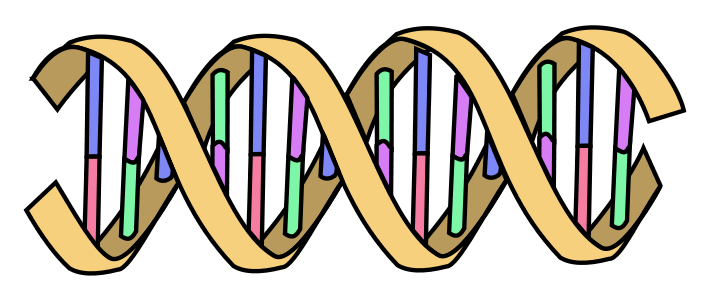
\includegraphics[width=0.8\textwidth]{images/DNA_Doppelhelix_Farbe.png}
	\caption[DNA Modell]{Ein farbcodiertes DNA Modell. Zu sehen ist das Zuckerphosphatrückgrat (gelb), das durch Basenpaare aus Adenin (A) und Thymin (T) oder Guanin (G) und Cytosin (C) verbunden ist.\cite{wikiFigDNA}}
	\label{fig:dna_doppelhelix}
\end{figure}

Das Konzept der DNA-Replikation wurde erstmals im Jahr 1958 von Meselson und Stahl beschrieben. Dabei handelt es sich um den Prozess, bei dem ein DNA-Molekül in zwei identische Kopien geteilt wird \cite{meselson1958replication}. Dieser Prozess beginnt mit der Denaturierung oder Trennung der Doppelhelix in zwei einzelne Stränge. Jeder dieser Einzelstränge dient dann als Vorlage für die Synthese eines neuen, komplementären Strangs. Dabei erkennt und bindet ein Enzym namens DNA-Polymerase die komplementären Basen (A zu T und C zu G) an den Einzelstrang. Dies führt zur Bildung einer exakten Kopie des ursprünglichen DNA-Strangs.

Diese Grundkenntnisse über die Struktur und den Replikationsmechanismus der DNA sind essenziell für das Verständnis der molekularen Genetik und können in der Nanotechnologie insbesondere bei der DNA-basierten Datenspeicherung genutzt werden. Die Fähigkeit der DNA zur Selbsterhaltung und Replikation ermöglicht die Erstellung genauer Kopien von Daten, was einen robusten und effizienten Mechanismus für die Datensicherung bietet.

\section{Self-Assembly}

\begin{figure}
	\centering 
	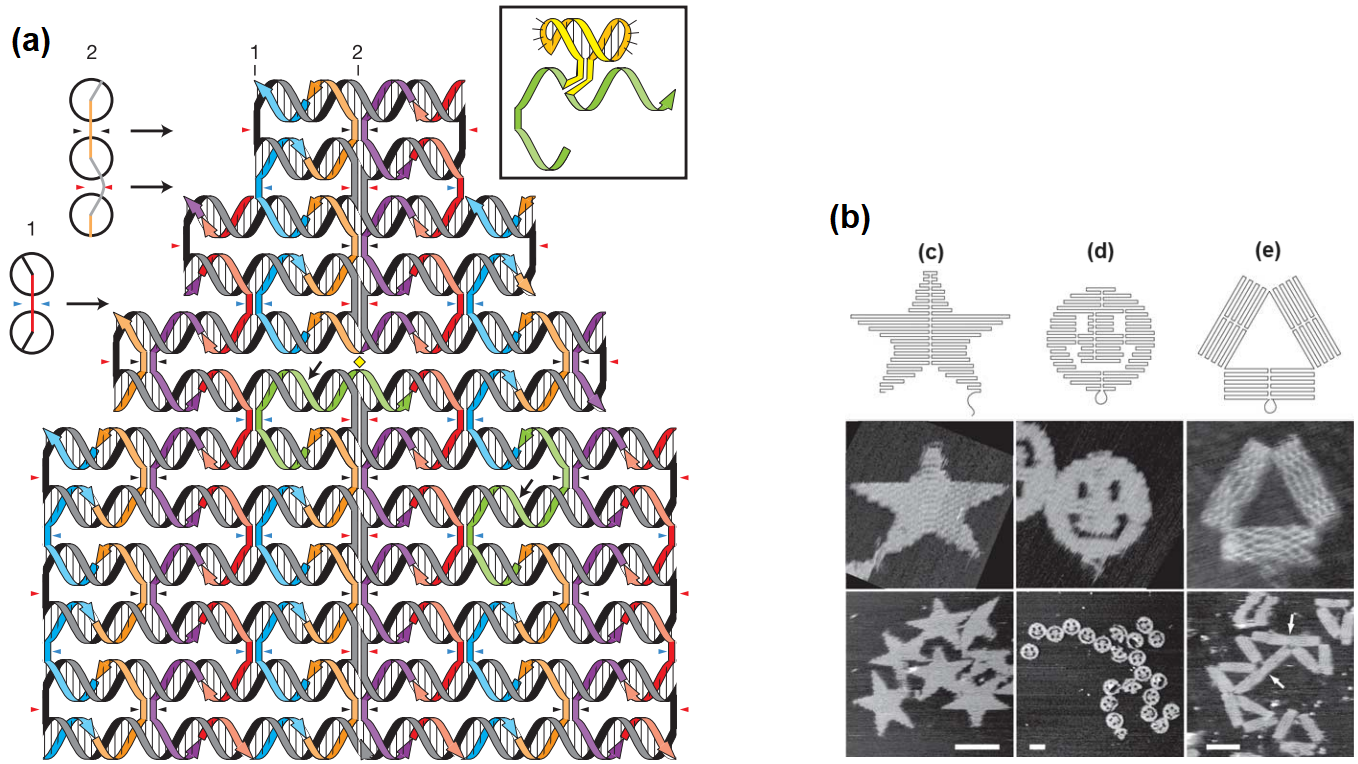
\includegraphics[width=0.9\textwidth]{DNA_Origami_Roth.png}
	\caption[DNA Origami]{DNA Origami aus der Arbeit von Rothemund \cite{rothemund2006origami}. 
	Dabei ist in (a) die Konstruktion eines langen DNA Strangs zu sehen, der durch Überkreuzungen und DNA Klammern in die gewollte Form gebracht werden kann. 
	In (b) wird ein Machbarkeitsbeweis gegeben. 
	Rothemund hat dafür verschiedene Strukturen erstellt. Von oben nach unten: Modell, Nahaufnahme einer Konstruktion und Aufnahme der Gesamtstruktur. 
	Hier abgebildet sind die folgenden Formen: ein Stern (c), ein Smiley (d) und ein Dreieck aus Rechtecken (e)}
	\label{fig:dna_origami}
\end{figure}

Für diese Arbeit von besonderem Interesse ist die \emph{DNA Self-Assembly}. 
Dabei wird DNA verwendet, um Strukturen zu bilden, die ohne weiteres äußeres Einwirken selbstständig und selbstorganisiert von den DNA-Strängen gebildet werden. Diese Technik bietet einen Bottom-Up Ansatz zur Bildung von komplexeren Strukturen auf der nanoskalaren Ebene. 

Die Grundlagen für DNA Self-Assembly legten Seeman et al. bereits in den 1980er Jahren. 
Es entstand die Idee davon, die Eigenschaften der Basenpaare gezielt zu nutzen, um die Moleküle in einer bestimmten Art und Weise anzuordnen.\cite{seeman1982dna}

Ein weiterer Grundbaustein der DNA Self-Assembly ist die Arbeit von Chad A. Mirkin et al. aus dem Jahr 1996. 
In ihrer Arbeit \glqq A DNA-based method for rationally assembling nanoparticles into macroscopic materials\grqq\, stellen die Forschenden eine Technik vor, durch die synthetisierte Goldnanopartikel durch DNA-Moleküle reversibel in spezifische Muster und Strukturen geordnet werden.\cite{mirkin1996assembling} 

Auf Basis dieser Grundbausteine wurden einige Ansätze zur DNA Self-Assembly entwickelt. 
Einer dieser Ansätze ist das \emph{DNA-Origami}. 
Erstmals vorgestellt im Jahr 2006 von Paul Rothemund, zeigte diese Technik, dass durch DNA Self-Assembly beliebige Strukturen zuverlässig konstruiert werden können. 
Ein DNA-Origami Molekül, sowie einige von Rothemund erstellte Strukturen sind in Abbildung~\ref{fig:dna_origami} zu sehen.\cite{rothemund2006origami}

%\begin{figure}
%	\centering
%	\begin{subfigure}{0.45\textwidth}
%		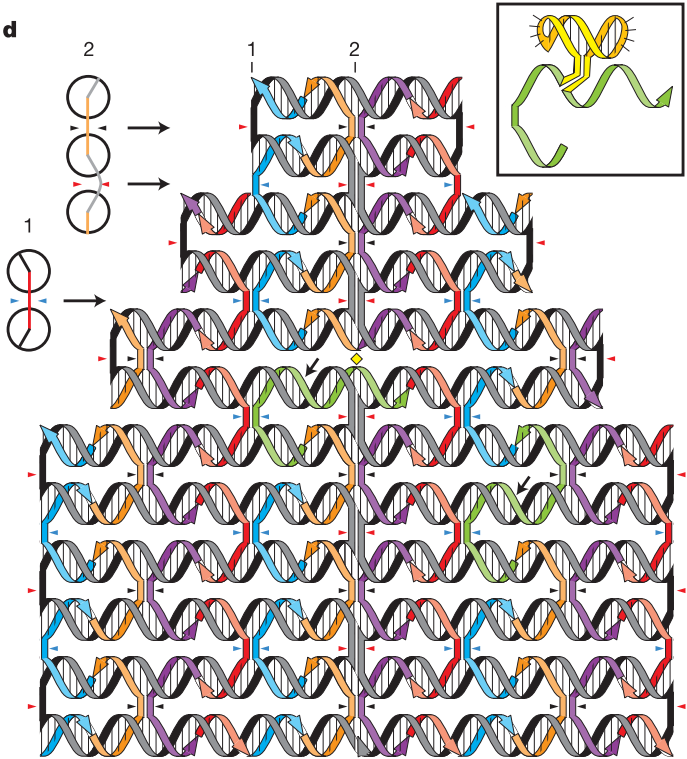
\includegraphics{DNA_Origami_Roth_A.png}
%		\subcaption{(a)}
%		\label{fig:dna_origami_a}
%	\end{subfigure}
%	\quad
%	\begin{subfigure}{0.45\textwidth}
%		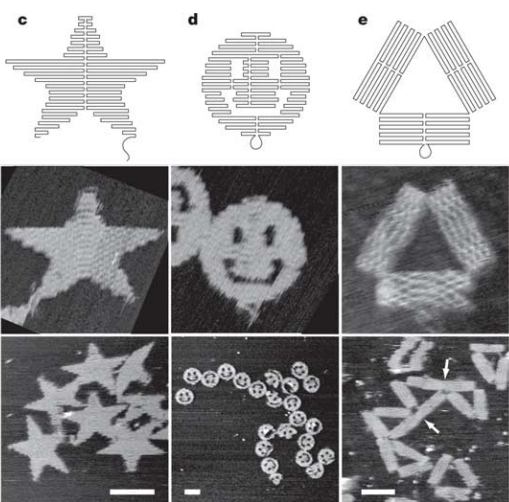
\includegraphics[width=\textwidth]{DNA_Origami_Roth_B.png}
%		\subcaption{(b)}
%		\label{fig:dna_origami_b}
%	\end{subfigure}
%	\caption{Test}
%	\label{fig:dna_origami}
%\end{figure}

Die von Rothemund vorgestellte Technik lässt sich ohne Probleme auch auf dreidimensionale Strukturen übertragen, wie die Arbeit von Ke et al. zeigt. \cite{ke2009origami3d}

\section{Tile-basierte Self-Assembly}

\begin{figure}
	\centering
	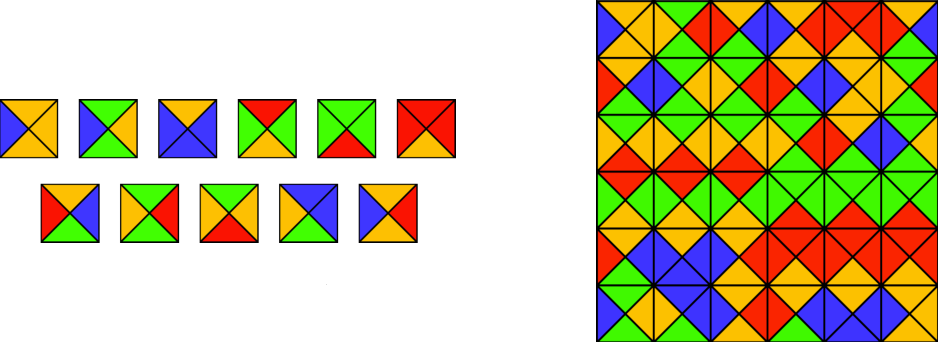
\includegraphics[width=0.65\textwidth]{images/Wang_Tiles.png}
	\caption[Wang Tiles]{Links Wang Tiles, die sich rechts zu einer lückenlosen Struktur zusammenfügen lassen.\cite{matsushima2016verfication}}
	\label{fig:wang_tiles}
\end{figure}

Basierend auf der zuvor beschriebenen Konstruktion von Nanostrukturen auf DNA-Basis, wird nun die \emph{Tile-basierte Self-Assembly} vorgestellt. 
Die theoretische Basis dieser Art der Self-Assembly sind die nach ihrem Erfinder benannten: die \emph{Wang Tiles}. 
Wang Tiles werden meist durch Quadrate mit vier farbigen Seiten dargestellt, wie in Abbildung~\ref{fig:wang_tiles} zu erkennen ist. 
Ein Tile aus einer Menge von Wang Tiles kann sich in einem $\mathbb{Z}^2$ Bereich nur mit anderen Tiles verbinden, wenn die Farben mit allen verbundenen Tiles übereinstimmen. 
Dieses Verhalten kann mit einem Puzzle verglichen werden und lässt sich direkt auf die Bindung von DNA-Tiles übertragen.\cite{wang1990tiles}

\begin{figure}
	\centering
	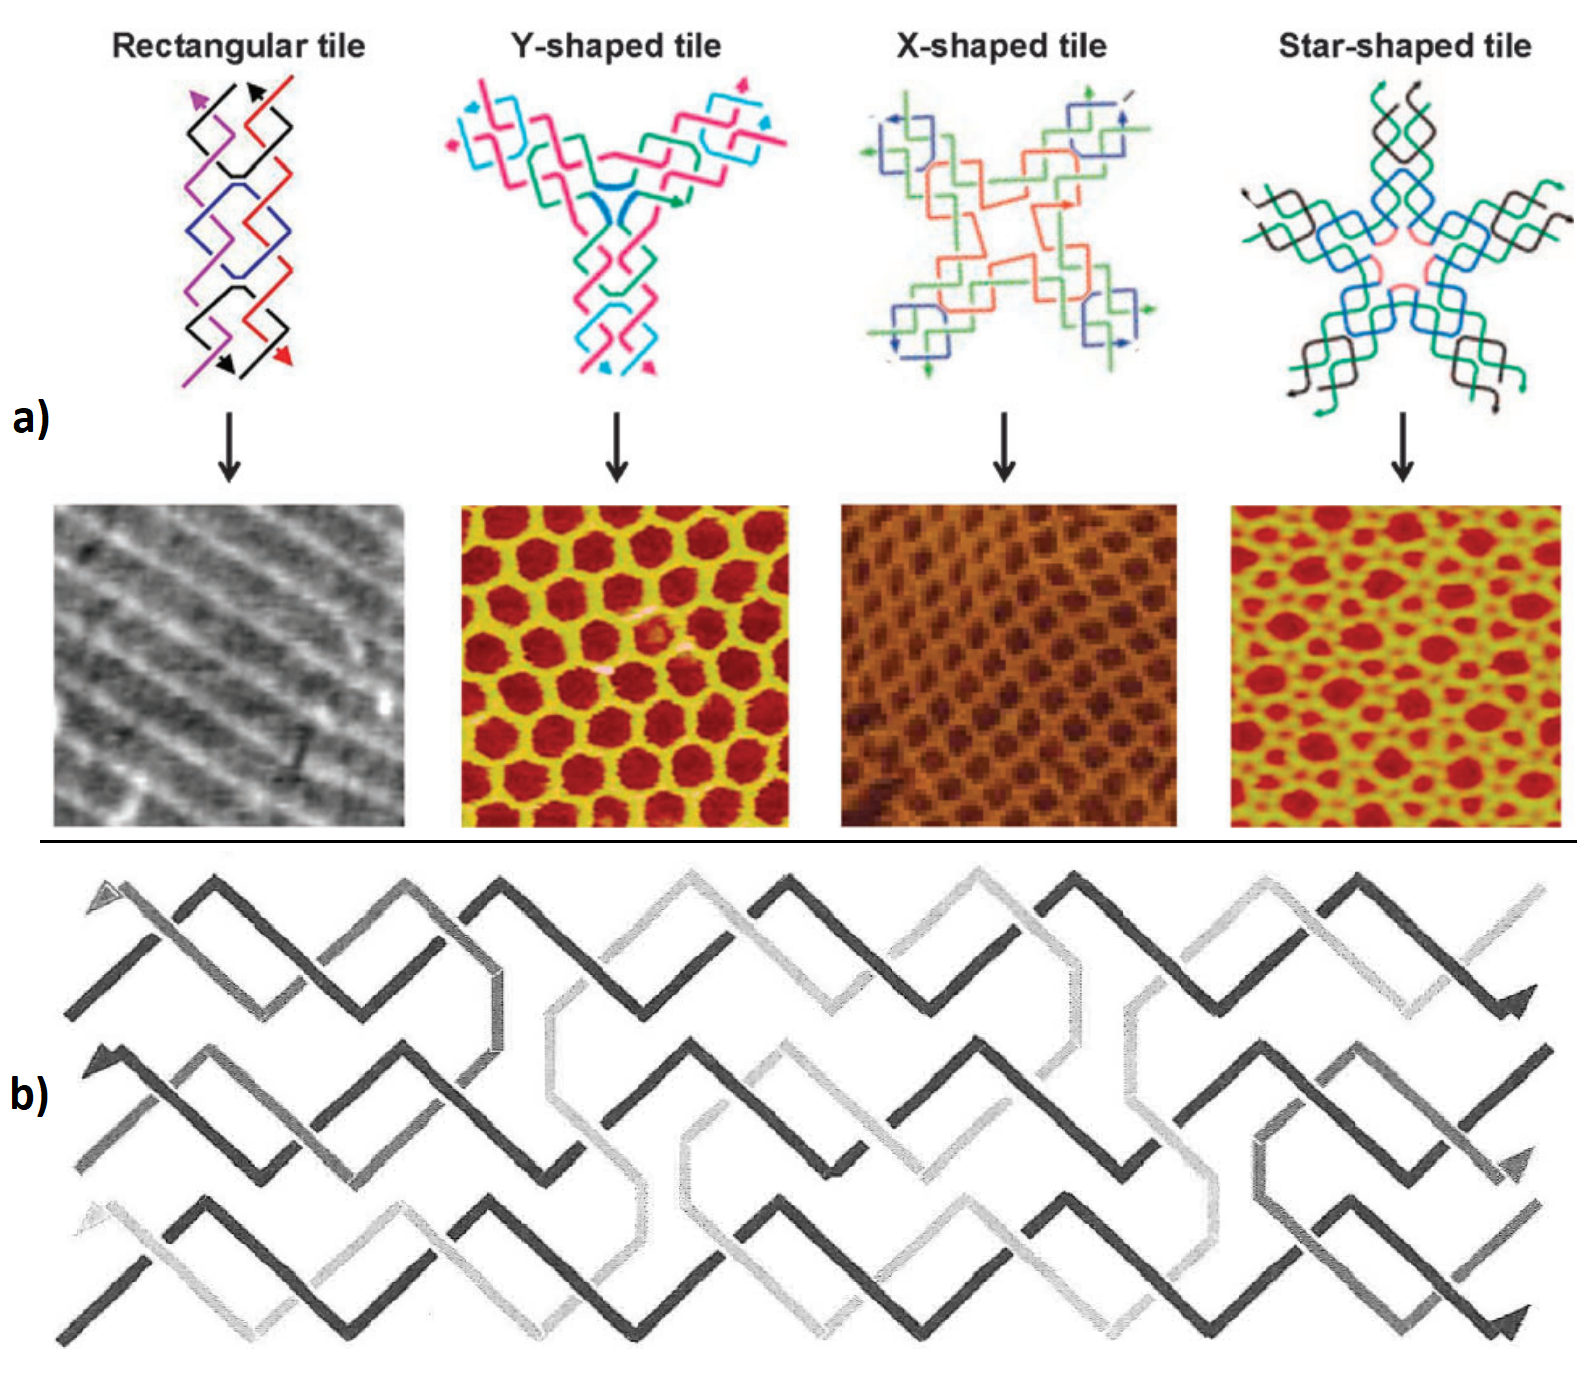
\includegraphics[width=0.8\textwidth]{images/DX_TX-Tiles.png}
	\caption[DX- und TX-Tiles]{Darstellung von zwei verschiedenen Tile-Strukturen. In a) ist das \emph{double-crossover-tile} (DX-tile) dargestellt \cite{roh2011materials}. Von links nach rechts ist eine Rechteckform, eine Y-Form, eine X-Form und eine Sternform zu sehen. Unten sind Aufnahmen der Strukturen unter einem Mikroskop dargestellt. In b) ist das Modell eines Triple-Crossover-Tiles (TX-Tiles) aus der Arbeit von Winfree et al. abgebildet \cite{winfree2000tx}. }
	\label{fig:dx_tx_tiles}
\end{figure}

Dafür werden im Weiteren einige DNA-Tiles vorgestellt. 
Es gibt verschiedene Arten von DNA-Tiles. In dieser Arbeit werden im Folgenden DX-Tiles, TX-Tiles und Holliday Junctions betrachtet. 
Diese sollten für einen allgemeinen Überblick von DNA-Tiles ausreichen, der in dieser Arbeit benötigt wird.

Die \emph{Double-Crossover-Tiles} (DX-Tiles) wurden 1993 von Fu und Seeman vorgestellt \cite{fu1993dx}. Dabei werden zwei Doppelstränge miteinander verwoben. 
Wie ganz links in Abbildung~\ref{fig:dx_tx_tiles} a) zu sehen ist, besteht die so entstandene Struktur aus zwei äußeren Strängen (orange und violett) und zwei inneren Strängen (schwarz und blau). 
Diese Verwebung von DNA bildet eine stabile Struktur. Dabei ist zu erkennen, dass das DX-Tile in dieser Grundform mehrere offene Stränge auf beiden Seiten hat. 
Es lassen sich damit weitere Strukturen wie zum Beispiel die Y-Form, X-Form oder Sternform bilden.
Auch ermöglichen die offenen Stränge die Verbindung von mehreren DX-Tiles, wodurch größere Strukturen durch Self-Assembly ermöglicht werden. Dies ist unten in Abbildung~\ref{fig:dx_tx_tiles} a) in den Aufnahmen der gebildeten Strukturen zu erkennen.

Eine Erweiterung der DX-Tiles bilden die \emph{Triple-Crossover-Tiles} (TX-Tiles). 
Vorgestellt wurden sie von Winfree et al. im Jahr 2000 \cite{winfree2000tx}. 
Durch die Verwebung von drei Doppelsträngen ist diese Struktur noch stabiler.
Außerdem ermöglicht das TX-Tile das Bilden von komplexeren Strukturen als das DX-Tile, da es einen größeren Abstand zwischen den offenen Enden aufweist.
Ein solches TX-Tile ist in Abbildung~\ref{fig:dx_tx_tiles} b) zu sehen.

Von besonderem Interesse für diese Arbeit sind die \emph{Holliday Junctions}. 
Von Seeman et al. \cite{kallenbach1983immobile} in ihrer Arbeit aus dem Jahr 1983 das erste Mal in einem Machbarkeitsbeweis vorgestellt, stammt diese Verbindung von DNA-Strängen aus der Feder von Holliday \cite{holliday1974molecular}.
Da diese Verbindung vier offene Enden in verschiedenen Richtungen hat, bietet sie sich gut zum Bilden von komplexeren Strukturen an. 
Wie in Abbildung~\ref{fig:holliday} zu erkennen ist, besteht eine Holliday Junction aus vier Strängen, die jeweils mit zwei anderen Strängen verbunden sind. 
Dabei entstehen vier offene Enden, die sich je nach Sequenz der Basenpaare nur mit ausgewählten anderen Strängen verbinden können. 
Aus Abbildung~\ref{fig:holliday} lässt sich ableiten, dass die Ausrichtung der vier offenen Enden variieren kann.
Für diese Arbeit wird jedoch nur die Ausrichtung in vier unterschiedliche Richtungen relevant sein.

Da somit der Prozess zur Bildung von DNA-Tiles vorgestellt wurde, kann im Weiteren die Modellierung und mathematische Darstellung der Tiles besprochen werden.

\begin{figure}
	\centering
	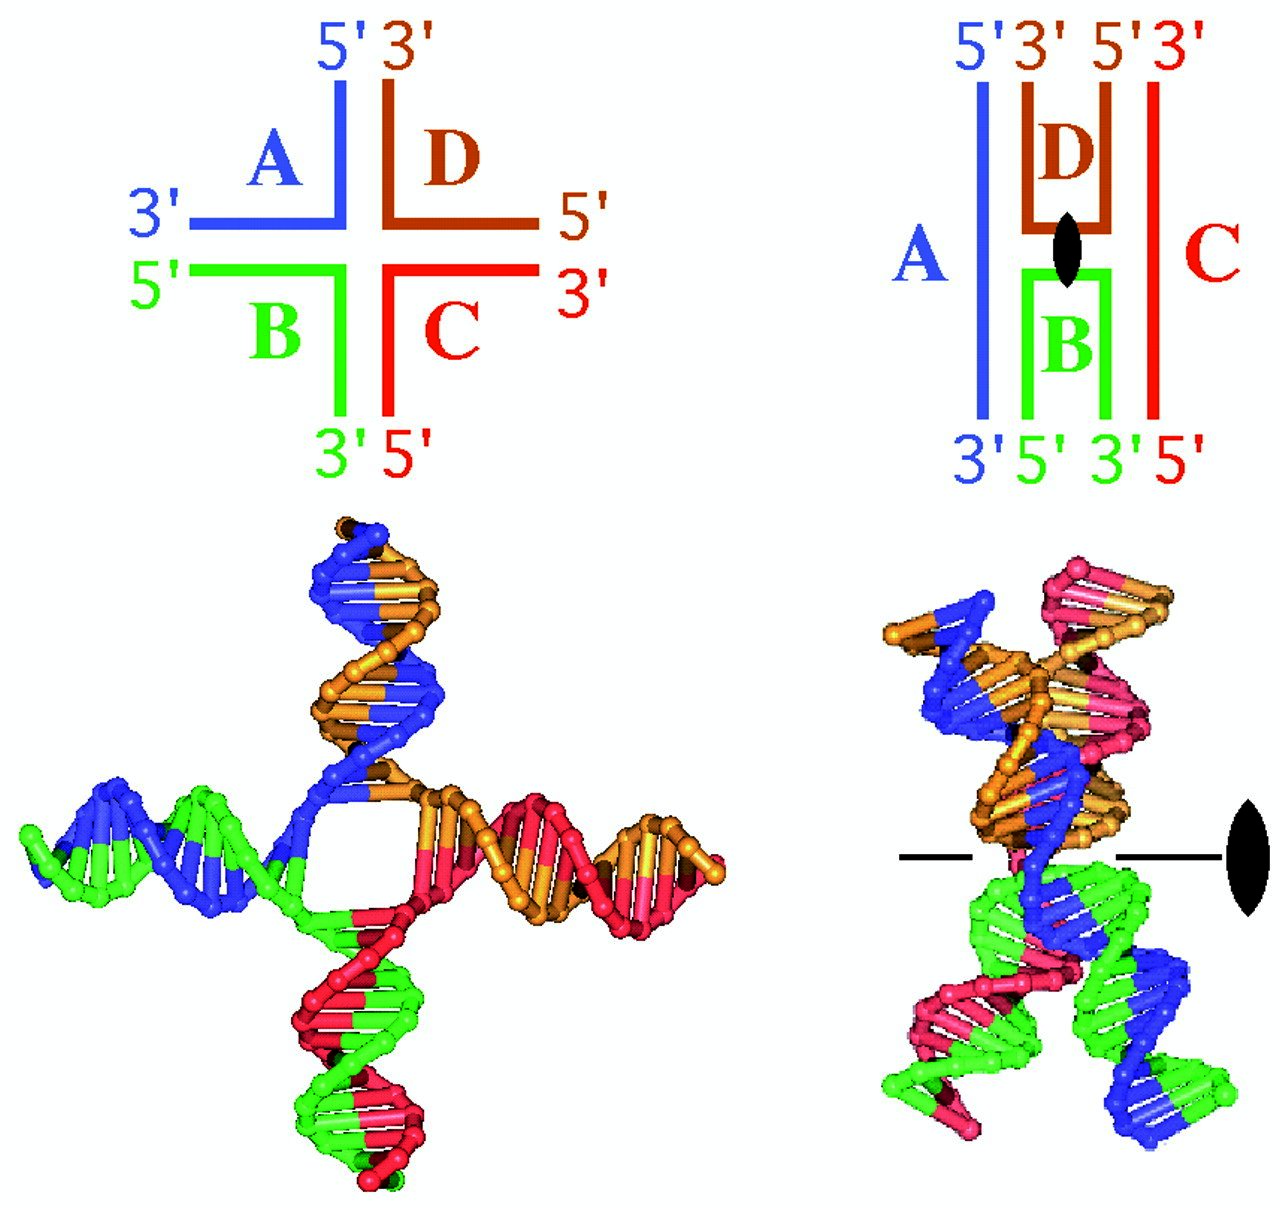
\includegraphics[width=0.5\textwidth]{images/Holliday_Junction.png}
	\caption[Holliday Junction]{Darstellung der Holliday Junction. Oben die Schemata von zwei möglichen Verbindungen. Unten die daraus entstandenen Modelle.\cite{brandt2000holliday}}
	\label{fig:holliday}
\end{figure}

\section{Nanogeräteklassen}
Um Modelle von Nanonetzwerken aus Nanogeräten und ihren Nachrichten erstellen zu können, müssen die verschiedenen Nanostrukturen zuerst definiert werden. Hierfür werden Definitionen aus der Arbeit von Büther et al. herangezogen \cite{buether2017formal}. Um Nanogeräte definieren zu können, müssen zuerst einige Kategorien festgelegt werden. 
Dazu zählen \emph{Aktuatoren} $A$, eine Komponente für die \emph{Kommunikation} mit anderen Geräten $C$, eine Komponente zur \emph{Informationsverarbeitung} $I$, eine Komponente zur \emph{Fortbewegung} $L$, ein \emph{Speicher} für Daten und Programme $M$\!, eine \emph{Energieversorgung} $P$\!, \emph{Sensoren} $S$ und \emph{Zeitgeber} $T$.

Um spezifische Nanogeräte definieren zu können, muss zu Beginn eine allgemeine Definition anhand der Kategorien zu Nanostrukturen gegeben werden. 

\begin{definition}
	Eine \emph{Nanostruktur} $\mathcal{N}_S = K_{opt}$ ist ein nanogroßes, künstliches Konstrukt, das konzipiert wurde, um eine spezifische Funktion in einer Umgebung $\Gamma$ zu erfüllen. Eine Nanostruktur besteht aus null oder mehr optionalen Komponenten $K_{opt}$. Diese sind definiert als $K_{opt} \subseteq \{A,C,I,L,M,P,S,T\}$.
\end{definition}

Eine einheitliche und klare Definition für \emph{Nanogröße} findet sich in der Literatur nicht, da sie sich je nach Angabe zwischen einem Nanometer und wenigen Mikrometern bewegt. 
Sie wird hier jedoch trotzdem verwendet, unter der Annahme, dass für den jeweiligen Anwendungsfall die Maximalgröße einer Nanostruktur beachtet wird.
Mit dieser allgemeinen Definition können im Weiteren Nanogeräte definiert werden.

\begin{definition}
	Ein \emph{Nanogerät} $\mathcal{N}_D = K_{mand} \cup K_{opt}$ ist eine Nanostruktur. Es besteht aus einer Menge notwendiger Komponenten $K_{mand} = \{P\}$ und einer Menge aus null oder mehr optionalen Komponenten $K_{opt} = \{A,C,I,L,M,S,T\}$.
\end{definition}

Um ein Nanogerät von einer passiven Nanostruktur unterscheiden zu können, benötigt das Nanogerät eine autarke Energieversorgung $P$. Die restlichen Komponenten sind wie auch bei den Nanostrukturen optional.
So können verschiedene Nanogeräte näher definiert werden.

\begin{definition}
	Eine \emph{Nanomaschine} $\mathcal{N}_M = K_{mand} \cup K_{opt}$ ist ein Nanogerät mit notwendigen Komponenten $K_{mand} = \{A,P\}$ und einer Menge aus null oder mehr optionalen Komponenten $K_{opt} \subseteq \{C,I,L,M,S,T\}$, in einer Umgebung $\Gamma$.
\end{definition}

\begin{definition}
	Ein \emph{Nanosensor} $\mathcal{N}_{Se} = K_{mand} \cup K_{opt}$ ist ein Nanogerät mit notwendigen Komponenten $K_{mand} = \{P,S\}$ und einer Menge aus null oder mehr optionalen Komponenten $K_{opt} \subseteq \{A,C,I,L,M,T\}$, in einer Umgebung $\Gamma$.
\end{definition}

\begin{definition}
	Ein \emph{Nanoknoten} $\mathcal{N}_{N} = K_{mand} \cup K_{opt}$ ist ein Nanogerät mit notwendigen Komponenten $K_{mand} = \{P,C\}$ und einer Menge aus null oder mehr optionalen Komponenten $K_{opt} \subseteq \{A,I,L,M,S,T\}$, in einer Umgebung $\Gamma$.
\end{definition}

Nanomaschinen, Nanosensoren und Nanoknoten sind in dieser Definition Nanogeräte, die entweder Aktuatoren $A$, Sensoren $S$ oder Kommunikationskomponenten $C$ besitzen. Analog zu diesen Definitionen lassen sich im Folgenden auch Nanoroboter definieren.

\begin{definition}
	Ein \emph{Nanoroboter} oder \emph{Nanobot} $\mathcal{N}_{R} = K_{mand} \cup K_{opt}$ ist ein programmierbares Nanogerät mit einem hohen Grad an Autonomie in einer Umgebung $\Gamma$. Es besteht aus einer Menge notwendiger Komponenten $K_{mand} = \{A,I,M,P,S\}$ und einer Menge aus null oder mehr optionalen Komponenten $K_{opt} \subseteq \{C,L,T\}$.
\end{definition}

Alle diese Nanostrukturen beziehungsweise Nanogeräte lassen sich mengentheoretisch mit ihren Überschneidungen in Abbildung~\ref{fig:nanostruktur} darstellen.

\begin{figure}
	\centering
	\resizebox{0.7\textwidth}{!}{
	\begin{tikzpicture}{scale=0.65}
		%% \draw[use as bounding box] (-4.2,-3.2) rectangle (4.2, 2.8);
		% \useasboundingbox (-4.2,-3.2) rectangle (4.2, 2.8);
		\fill[
		pattern=north east lines, pattern color=blue!30!white]
		(0,-1.6) ellipse[x radius=3, y radius=1.2];
		\fill[
		pattern=vertical lines, pattern color=lightgray]
		(-1.1,0) ellipse[x radius=3, y radius=1.7];
		\fill[
		pattern=horizontal lines, pattern color=green]
		(1.1,0) ellipse[x radius=3, y radius=1.7];
		\fill[
		pattern=crosshatch dots, pattern color=black!40!white]
		(0, 0) ellipse[x radius=1.7, y radius=1];
		\fill[
		pattern=crosshatch dots, pattern color=green]
		(-3.6,2.3) ellipse[x radius=1.35, y radius=1.1];
	
		\draw (-3.6,2.3) ellipse[x radius=1.35, y radius=1.1];
		\draw (0,-0.2) ellipse[x radius=6, y radius=5];
		\draw (0,-0.2) ellipse[x radius=5.2, y radius=4];
		\draw (0,-0.2) ellipse[x radius=4.2, y radius=3];
		\draw (0,-1.6) ellipse[x radius=3, y radius=1.2];
		\draw (-1.1,0) ellipse[x radius=3, y radius=1.7];
		\draw (1.1,0) ellipse[x radius=3, y radius=1.7];
		\draw (0,0) ellipse[x radius=1.7, y radius=1];
	
		\node[align=center] at (-3.55,2.35) (A2) { \contour{white}{Moleküle}\\\contour{white}{Cluster}\\\contour{white}{Fullerene} \\\contour{white}{Nanopartikel} };
		\node at (0,4.2) (A1) {Nanoobjekt $\mathcal{N}_{O}$};
		\node at (0,3.2) (A0) {Nanostruktur $\mathcal{N}_{S}$};
		\node at (0,2.2) (A) {Nanogerät $\mathcal{N}_D$};
		\node[align=center] at (-3,0) (B) { \contour{white}{Nano-}\\ \contour{white}{sensor $\mathcal{N}_{So}$}};
		\node[align=center] at (3,0) (C) { \contour{white}{Nano-}\\ \contour{white}{maschine $\mathcal{N}_M$}};
		\node at (0,0.1) (D) {\contour{white}{Nanoroboter $\mathcal{N}_R$}};
		\node at (0,-2.2) (E) {\contour{white}{Nanoknoten $\mathcal{N}_N$}};
	\end{tikzpicture}}
	\caption[Nanostrukturen Venn-Diagramm]{Venn-Diagramm verschiedener Nanostrukturen und ihren Überschneidungen.\cite{lau2020phd}}
	\label{fig:nanostruktur}
	\end{figure} 

\section{Tile-Assembly Modelle}
Neben der Definition von Nanostrukturen müssen für diese Arbeit eindeutig definierte Modelle und Modellierungverfahren vorgestellt werden, um Nanonetzwerke modellieren zu können.
Dafür werden in den folgenden Absätzen das \emph{Abstract Tile-Assembly Model} (aTAM), das \emph{Kinetic Tile-Assembly Model} (kTAM), das \emph{Two-Handed Tile-Assembly Model} (2HAM) und das \emph{Kinetic Two-Handed Tile-Assembly Model} (kTHAM) definiert. Um diese Modelle vorstellen zu können, müssen jedoch zu Beginn einige grundlegenden Begriffe definiert werden. Alle folgenden Notationen und Definitionen basieren auf den Arbeiten von Lutz et al. \cite{lathrop2009strict} und Patitz \cite{patitz2014introduction}.

\begin{definition}
	Ein $n$-dimensionales \emph{Tile} $t_n$ ist ein Objekt in $\mathbb{Z}^n$ mit Einheitslänge und 90 Grad Winkeln. 
	Eine \emph{Seite} eines Tiles $t_n$ ist durch einen Vektor $u_i \in U_t \subseteq \mathbb{Z}^n$ definiert. $U_t$ ist eine Menge von eindeutigen Richtungsvektoren. 
	Der Gegenvektor $-u_i$ beschreibt die gegenüberliegende Seite von $u_i$ in derselben Dimension. Der Vektor $u_i$ hat genau einen Eintrag, der ungleich $0$ ist. Die Seiten eines Tiles sind durch folgende Relation definiert:
	\begin{align*}
		\text{Seite: }t_n \mapsto \underbrace{U_t\times U_t\times \dots\times U_t}_n
	\end{align*} 
\end{definition}

In dieser Arbeit werden hauptsächlich zweidimensionale Tiles von Bedeutung sein. Daher wird im Folgenden immer von zweidimensionalen Tiles gesprochen, wenn die Dimension nicht angegeben ist.

In jedem \emph{Tile Assembly System (TAS)} gibt es eindeutig definierte Regeln, durch die sich zwei Tiles miteinander verbinden können. Dafür wird Folgendes definiert:

\begin{definition}
	Ein \emph{Kleber} oder \emph{Glue} $g\in G$, wobei $G$ die Menge der möglichen Kleber beschreibt, ist durch einen \emph{Bezeichner} oder ein \emph{Label} $\mathcal{L}_g\in\Sigma^*$ definiert, wobei $\Sigma$ ein Alphabet ist und $s\in\mathbb{N}$ eine \emph{Kleberstärke} mit den Funktionen:
	\begin{align*}
		\text{label : }& G\mapsto\Sigma^* \\
		\text{strength : }& G\mapsto\mathbb{N}
	\end{align*}
\end{definition}
\begin{definition}
	Zwei Tiles $t$ und $t'$, die durch $v_t$ und $v_{t'}\in\mathbb{Z}^n$ definierte Orte belegen, sind genau dann benachbart, wenn $|v_t-v_{t'}| = 1$ und der resultierende Vektor $e = v_t-v_{t'}$ genau ein Element ungleich $0$ hat.
\end{definition}
Ein Tile kann auf allen Seiten immer nur genau einen oder keinen Nachbarn haben.
\begin{definition}
	Die \emph{Temperatur} $\tau$ eines TAS beschreibt die minimale Stärke des Klebers $s$ für eine stabile Verbindung.
\end{definition}
Damit ein Tile in einem TAS eine stabile Verbindung aufbauen kann, muss die absolute Kleberstärke des Tiles mindestens der Temperatur des Systems entsprechen. Die absolute Kleberstärke ergibt sich aus der Summe aller Kleberstärken des Tiles mit den verbundenen anderen Tiles.
\begin{definition}
	Ein \emph{$n$-dimensionaler Tiletyp} $T_n$ ist eine Schablone für ein Tile $t_n$. Ein $n$ dimensionaler Tiletyp wird durch einen Bezeichner $\mathcal{L}_T\in\Sigma^*$ und einer Menge von Klebern $g_i\in G$ definiert. Ein Kleber befindet sich an jeder Seite $u_{t,i}\in U_t$ von $t_n$. Folgende Funktionen sind jedem Tiletyp zugeordnet:
	\begin{align*}
		\text{glue : }& T_n\times U_t\mapsto G \\
		\text{strength : }& g\in G \mapsto \mathbb{N}
	\end{align*}
\end{definition} 
Eine so definierte Tileschablone kann wie in Abbildung~\ref{fig:dna_tile_math} dargestellt werden. 
Hierbei bekommt jedes Tile eine eindeutige Beschriftung, in diesem Beispiel ist es die \glqq 1\grqq.
Auf den vier Seiten des Tile kann so mit einer weiteren Beschriftung die \emph{Farbe}, der \emph{Kleberbezeichner}, dargestellt werden.
Der Kleberbezeichner wird durch die Sequenz der Basenpaare an den offenen Enden definiert. Dies ist in Abbildung~\ref{fig:dna_tile_bio} zu erkennen. 
Nur wenn der Kleberbezeichner von zwei Tiles gleich ist, können sich die Tiles im Zuge der Self-Assembly verbinden. 
Im Beispiel aus Abbildung~\ref{fig:dna_tile_math} sind die Kleberbezeichner mit den Beschriftungen \glqq A,B,C,D\grqq\, gegeben. 
Außerdem wird die Kleberstärke des Tiles durch ausgefüllte schwarze Boxen an den Seiten des Tiles dargestellt. 
Dabei entscheidet die Menge an schwarzen Boxen die Stärke des Klebers.

Die Verbindung zweier Tiles funktioniert wie folgt:
\begin{definition}
	Zwei Tiles $t$ und $t'$ \emph{binden korrekt} bei Temperatur $\tau$, wenn folgende Bedingungen gelten:
	\begin{align*}
		&(1)~ t \text{ und } t' \text{ sind benachbart.}\\
		&(2)~ \exists u_i\in U_t: label(glue(t,u_i)) = label(glue(t',-u_i)) \\
		&\qquad\qquad\quad~~\land strength(glue(t,u_i)) \geq \tau \land strength(glue(t',-u_i)) \geq \tau
	\end{align*}
	Wenn eine der beiden Bedingungen $(1)$ oder $(2)$ verletzt wird, wird diese Verbindung \emph{Error} oder \emph{false} genannt.
\end{definition} 

\begin{figure}
	\centering
	\begin{tikzpicture}[scale=2.0]
		\tileBsp{1}{1}
	\end{tikzpicture}
	\caption[Mathematisches Schema eines DNA-Tiles]{Mathematisches Schema eines DNA-Tiles. Die schwarzen Boxen stellen dabei die Stärke des Klebers auf den jeweiligen Seiten dar (hier 1). Die Beschriftungen (A, B, C, D) stellen die Farbe oder die Kleberbezeichner dar. Mit der \glqq 1\grqq\, wird das Tile beschriftet und gibt damit dem Tile einen Namen, um Beschreibungen und Analysen einfacher zu machen.}
	\label{fig:dna_tile_math}
\end{figure}


\begin{figure}
	\centering
	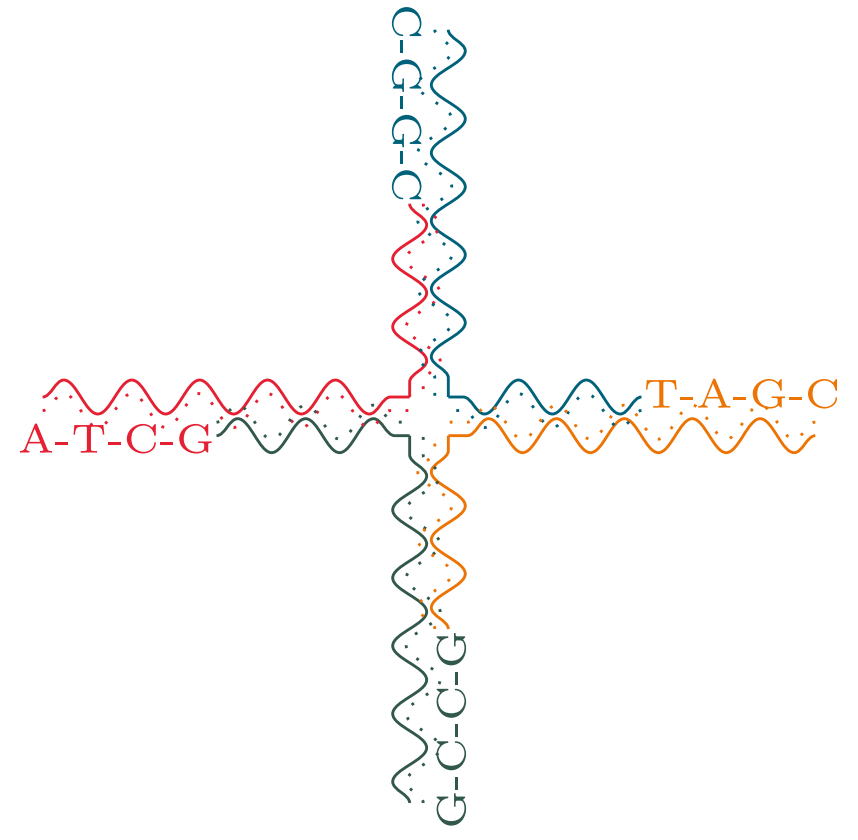
\includegraphics[width=0.5\textwidth]{images/DNA_Tile.png}
	\caption[Biologisches Schema einer Holliday Junction]{Biologisches Schema einer Holliday Junction, deren vier offenen Enden so gewählt wurden, dass sie sich oben und unten sowie rechts und links mit sich selbst verbinden kann.\cite{lau2019dnatiles}}
	\label{fig:dna_tile_bio}
\end{figure}
Die Verbindung von mehreren Tiles wird \emph{Assembly} genannt.

\begin{definition}
	Eine n-dimensionale \emph{Tile Assembly} oder \emph{Assembly} ist eine partielle Funktion $\alpha:\mathbb{Z}^n\mapsto T$ mit $T$ als Menge von n-dimensionalen Tiles. Eine Assembly $\alpha$ ist \emph{$\tau$-stabil}, wenn kein Tile $t_n\in T$ aus der Assembly entfernt werden kann, ohne dafür Kleber der Stärke $\tau\in\mathbb{N}$ entfernen zu müssen. 
\end{definition}

\begin{definition}
	Die \emph{Grenze} einer Assembly $\alpha$ ist eine Teilmenge von $\alpha$. Diese Menge enthält alle Tiles mit mindestens einem freien Nachbar-Tile.
\end{definition}

\begin{definition}
	Die \emph{Wachstumsfront} einer $n$-dimensionalen Assembly $\alpha$ ist eine Teilmenge von $\mathbb{Z}^n$. Eine Stelle ist nur dann Teil der Wachstumsfront, wenn folgende Bedingungen eintreffen:
	\begin{align*}
		&(1) \text{ Die Stelle ist nicht belegt.}\\
		&(2) \text{ Die Stelle liegt an der Grenze der Assembly.}\\
		&(3) \text{ Die benachbarte Seite des Tiles an der Grenze hat eine minimale Kleberstärke } 1.
	\end{align*}
\end{definition}

In einer gegebenen Assembly ändern sich sowohl die Grenzlinie als auch die Wachstumsfront kontinuierlich durch die Prozesse des Hinzufügens und Entfernens von Tiles. Wenn eine Assembly zu einem Zeitpunkt keine offenen Enden mit einer Kleberstärke von größer oder gleich eins aufweist, dann existiert für diese Assembly keine Wachstumsfront. Trotz dieser dynamischen Veränderungen verfügt jede Assembly zu jedem Zeitpunkt über eine klar definierte Grenze.

Das erste Tile einer Assembly, bezeichnet als $\alpha_0$ zum initialen Zeitpunkt $t=0$, erhält die Bezeichnungen \emph{Seed-Assembly} oder \emph{Seed-Tile} und wird als $\sigma$ gekennzeichnet. An der Wachstumsfront dieser Seed-Assembly kann die Anbindung weiterer Tiles auf einer nichtdeterministischen Basis erfolgen.

Im Folgenden werden die Modelle definiert, die in Kapitel~\ref{cha:simulationen} zur Simulation und Evaluation der Ergebnisse verwendet werden.

\begin{definition}
	Ein \emph{Tile Assembly Model (TAM)} ist ein Tupel $\mathcal{T}_\tau = (T,\sigma,\tau)$, mit $T$ als endliche Menge von Tiles (auch \emph{Tileset} genannt), $\sigma$ der Seed-Assembly und $\tau\in\mathbb{N}$ als Temperatur des TAM. 
\end{definition}

\begin{definition}
	$\mathcal{A}[\mathcal{T}]$ ist die Menge aller terminierten Assemblies, die als Ergebnis eines TAM in endlicher Zeit erreicht werden können. 
	Eine Assembly $\alpha\in\mathcal{A}[\mathcal{T}]$ gilt als \emph{terminiert $(\alpha_{\square})$}, wenn kein weiteres $\tau$-stabiles Tile in der Assembly hinzugefügt werden kann.
\end{definition}

\begin{definition}
	Sei $\alpha_i$ eine durch ein TAM definierte Assembly. Eine \emph{Assembly Sequenz} ist eine Sequenz $S=<\alpha_0,\alpha_1,\dots>$, wobei $\alpha_{i+1}$ die Assembly $\alpha_i$ mit einem weiteren hinzugefügten Tile darstellt. 
	Wenn die Sequenz $s$ endlich ist, dann wird das letzte Element der Sequenz \emph{Ergebnis $\alpha_\square$} oder \emph{terminiert} genannt.
\end{definition}

Aus diesen Definitionen kann so das erste Modell, das \emph{Abstract Tile Assembly Model (aTAM)} definiert werden:

\begin{definition}
	Sei $T$ eine Menge von Tiles, die nicht rotiert werden können. Sei $\sigma$ eine Seed-Assembly. Dann ist das Tupel $\mathcal{A} =(T,\sigma,\tau)$ ein Abstract Tile Assembly Model (aTAM) mit Temperatur $\tau$\!. In einem aTAM kann immer nur ein einzelnes Tile zu einem Zeitpunkt hinzugefügt werden. Des Weiteren können Tiles nicht wieder aus der Assembly entfernt werden.
\end{definition}

Das aTAM ist das einfachste in dieser Arbeit betrachtete Modell der Tile-basierten Assembly. 
Als Beispiel für solch eine Assembly dient Abbildung~\ref{fig:assembly_bsp}. 
Zu sehen ist ein aTAM $\mathcal{A} = (T,S,\tau)$ mit der Menge der Tiles $T=\{ \sigma,a,b,c\}$ und der Temperatur $\tau = 2$. 
Das Tileset ist links in der Abbildung dargestellt. Die Assembly Sequenz $S = <\alpha_0,\alpha_1,\alpha_2,\alpha_3>$ ist rechts zu erkennen. Da das Beispiel mit im aTAM durchgeführt wird, ist $\alpha_3=\alpha_\square$, da bei einer Temperatur von zwei keine weiteren Tiles mit dem Bezeichner \glqq C\grqq\, an der Wachstumsfront hinzugefügt werden können. Diese Verbindungen wären nicht $\tau$-stabil.

\begin{figure}
	\centering 
	\begin{tikzpicture}[scale=1.1]
		\tileAssemblyC{1}{2.5}
		\tileAssemblySigma{1}{1}
		\tileAssemblyA{2.5}{2.5}
		\tileAssemblyB{2.5}{1}
		%%%
		\node[scale = 1.2] at (4.5,3) {$\alpha_0$};
		\tileAssemblySigma{4.5}{1}
		%%%
		\node[scale = 1.2] at (6.5,3) {$\alpha_1$};
		\node[scale = 1.2] at (5.5,1.6) {$\rightarrow$};
		\tileAssemblyA{6.5}{2.2}
		\tileAssemblySigma{6.5}{1}
		%%%
		\node[scale = 1.2] at (9.1,3) {$\alpha_2$};
		\node[scale = 1.2] at (7.5,1.6) {$\rightarrow$};
		\tileAssemblyA{9.7}{2.2}
		\tileAssemblySigma{9.7}{1}
		\tileAssemblyB{8.5}{1}
		%%%
		\node[scale = 1.2] at (12.3,3) {$\alpha_3$};
		\node[scale = 1.2] at (10.7,1.6) {$\rightarrow$};
		\tileAssemblyA{12.9}{2.2}
		\tileAssemblySigma{12.9}{1}
		\tileAssemblyB{11.7}{1}
		\tileAssemblyC{11.7}{2.2}
	\end{tikzpicture}
	\caption[Beispiel Assembly]{Beispiel Assembly von vier Tiles (links) in Sequenz bei Temperatur $\tau = 2$. Im ersten Schritt $\alpha_0$ liegt nur die Seed-Assembly vor. In Schritten $\alpha_1$ und $\alpha_2$ binden sich nichtdeterministisch die Tiles \glqq A\grqq\, und \glqq B\grqq\, an der Seed-Assembly an. In Schritt $\alpha_3$ bindet sich so das Tile \glqq C\grqq. Da bei Temperatur zwei keine stabile Verbindung von zwei \glqq C\grqq-Tiles möglich ist, ist $\alpha_3$ das Resultat der Assembly.\cite{lau2019dnatiles}}
	\label{fig:assembly_bsp}
\end{figure}

Durch die Annahme, dass sich keine Tiles wieder aus der Assembly entfernen können und Schritt für Schritt immer nur ein Tile hinzugefügt werden kann, werden einige Grenzfälle in aTAM nicht betrachtet. Im Beispiel aus Abbildung~\ref{fig:assembly_bsp} könnte zum Beispiel durch Hinzufügen von drei \glqq C\grqq\, Tiles, wieder eine stabile Verbindung gebildet werden. Diese Betrachtung gibt es in aTAM jedoch nicht.
Dadurch gilt dieses Modellierungsverfahren als simpel, aber nicht realitätsnah.
Ein Modellierungsverfahren, das näher an der Realität und näher am Verhalten von DNA im Vorgang der Self-Assembly liegt, ist das \emph{Kinetic Tile-Assembly Model (kTAM)}.
Durch diese Eigenschaft wird kTAM die größte Rolle bei der Simulation und Auswertung von Kommunikationsprotokollen in dieser Arbeit spielen.
Im Gegensatz zu aTAM können sich in kTAM verbundene Tiles von der Assembly lösen. 
Außerdem ist es möglich, dass ein Tile sich an einer falschen Stelle bindet. 
Dies ist in aTAM nicht möglich. 
Um die Verbindung und Trennung von Tiles in kTAM darstellen zu können, muss jedoch erst einmal die \emph{Forward Rate} und \emph{Backward Rate} definiert werden. 

\begin{definition}
	Sei $\mathcal{T}_\tau$ ein TAM, $\sigma$ ein nicht leere Seed-Assembly und $T$ eine Menge an Tiles. Die \emph{Forward Rate} $r_f$, mit welcher Tiles $t$ in der Assembly hinzugefügt werden, wird wie folgt definiert:
	\begin{align*}
		r_f(t) = k_fe^{-G_{mc}}.
	\end{align*}
	$k_f$ beschreibt hier das Timing des Systems, $G_{mc}$ die benötigte Energie, um ein Tile zu binden \emph{(Binding Cost)}. Dabei gilt $G_{mc} > 0$.
\end{definition}
\begin{definition}
	Analog zur Forward Rate ist die \emph{Backward Rate} wie folgt definiert:
	\begin{align*}
		r_{r,b}(t) = k_fe^{-G_{se}}.
	\end{align*}
	Sie beschreibt mit welcher Rate sich Verbindungen in einer Assembly wieder lösen. $G_{se}$ beschreibt hierbei die benötigte Energie zum Lösen der Verbindung \emph{(Bond Breaking Cost)}. Durch $b$ wird die Anzahl der Verbindungen des Tiles angegeben.
\end{definition}

Daraus lässt sich im Weiteren das kTAM definieren:
\begin{definition}
	Sei $\sigma$ eine nicht leere Seed-Assembly, $T$ eine Tileset, $r_{r,b}$ die Backward Rate und $r_f$ Forward Rate. Dann ist ein Kinetic Tile Assembly Model wie folgt definiert:
	\begin{align*}
		\mathcal{K} = (T,\sigma,r_{r,b},r_f)
	\end{align*}
\end{definition}
Im kTAM leitet sich die Temperatur aus dem Verhältnis zwischen $G_{mc}$ (Binding Cost) und $G_{se}$ (Bond Breaking Cost) ab. Da die Temperatur selbst nicht explizit spezifiziert wird, wird sie implizit durch die zuvor definierten Forward und Backward Rates repräsentiert.
In kTAM wird in jedem Schritt ein nicht deterministisch ausgewähltes Tile an einer nicht deterministisch festgelegten Stelle der Assembly hinzugefügt. Eine korrekte Positionierung ist dabei um den Faktor $e^{G_{se}}$ wahrscheinlicher als eine falsche Positionierung. Außerdem ist bei falscher Positionierung die Wahrscheinlichkeit größer, dass durch die Backward Rate diese Verbindung wieder aufgelöst wird.

Ein weiteres realitätsnäheres Modell ist das \emph{Two-Handed Tile-Assembly Model (2HAM)}. 
Im 2HAM gibt es keine Seed-Assembly. Solange die Temperaturbeschränkungen eingehalten werden, kann jedes Tile und jede Assembly in allen Schritten mit anderen Assemblies interagieren. Dadurch wird eine Art Potenzmenge aller möglichen Assemblies gebildet.
Das Entfernen einer einzelnen Seed-Assembly, sowie das Verhalten beim Erzeugen einer Assembly macht dieses Modellierungsverfahren realitätsnäher.
Für die formale Definition des 2HAM müssen zunächst einige Definitionen gegeben werden:

\begin{definition}
	Zwei Assemblies $\alpha$ und $\beta$ sind disjunkt, wenn für alle Stellen in $\alpha$ und $\beta$ gilt: $\alpha\cap\beta = \emptyset$. Eine Assembly besteht immer aus mindestens einem Tile.
\end{definition}

\begin{definition}
	Der Zustand $S$ eines Tilesets $T$ ist eine Multimenge von Assemblies, für die Folgendes gilt:
	\begin{enumerate}
		\item Alle Assemblies $\alpha\in S$ sind $\tau$-stabil. Es müssen $\tau$ Kleber entfernt werden, damit sich die Assembly auflöst. 
		\item Alle Assemblies $\alpha\in S$ können aus der Menge $T$ durch korrekte Vereinigung gebildet werden.
	\end{enumerate}
\end{definition}

Der Zustand $S$ von $T$ ist als Multimenge definiert, da eine Verbindung eines Tiles mit sich selbst möglich sein muss. 
So müssen einige Elemente mehrfach in der Menge vorkommen. 
Zwei Asssemblies $\alpha$ und $\beta$ bilden eine \emph{korrekte Verbindung}, wenn ihre Verbindung $\tau$-stabil ist und $\alpha$ und $\beta$ disjunkt sind.

\begin{definition}
	Ein \emph{Two-Handed Tile Assembly Model (2HAM)} ist wie folgt definiert: Ein 2HAM ist ein Tupel $\mathcal{H} = (T,S_0,\tau)$ mit dem Tileset $T$, dem Startzustand $S_0$ und der Temperatur $\tau$.
\end{definition}
\begin{definition}
	Sei $\mathcal{H} = (T,S_0,\tau)$ ein 2HAM. Die Assembly Sequenz eines 2HAM ist eine Sequenz von Zuständen $S=<S_0,\dots,S_k>$ mit $k=\{1,\dots,\infty\}$. $S_{i+1}$ wird aus $S_i$ gebildet, indem alle möglichen Vereinigungen auf Assemblies $s,s'\in S_i$ durchgeführt werden.
\end{definition}
\begin{definition}
	Sei $\mathcal{H} = (T,S_0,\tau)$ ein 2HAM. Ein Zustand $S_i$ ist terminierend, wenn $S_{i+1}$ nach allen möglichen Vereinigungen äquivalent zu $S_i$ bleibt.
\end{definition}

Alle Definitionen zu aTAM, kTAM und 2HAM bis hier stammen aus der Arbeit von Patitz \cite{patitz2014introduction} und der Arbeit von Lathrop et al.\cite{lathrop2009strict}. Alle jetzt folgenden Definitionen zum \emph{Kinetic Two-Handed Tile-Assembly Model (kTHAM)} stammen aus der Arbeit von Kaussow in Zusammenarbeit mit Lau \cite{kaussow2022thesis}.

"Das Kinetic Two-Handed Tile-Assembly Model kombiniert die realitätsnahen Merkmale von 2HAM und kTAM. Analog zum 2HAM gibt es keine Seed-Assembly. Gleichzeitig, ähnlich wie im kTAM, können sich Verbindungen und Vereinigungen bilden, die nicht $\tau$-stabil sind, und bereits gebildete Verbindungen können in späteren Schritten wieder aufgelöst werden.

Dafür müssen wieder einige Definitionen aufgestellt werden.

\begin{definition}
	Eine \emph{korrekte Vereinigung} von zwei Assemblies $\alpha$ und $\beta$ im kTHAM ist eine Vereinigung, in der $\alpha$ und $\beta$ disjunkt sind.
\end{definition}

\begin{definition}
	Ein Zustand $S=\{A_S,C_S\}$ eines Tilesets $T$ ist ein Tupel von Multimengen von Assemblies und ein Vektor für ihre Nummer im kTHAM. Für das Tupel gilt Folgendes:
	\begin{enumerate}
		\item Alle Assemblies $A_S$ können aus $T$ durch korrekte Vereinigungen gebildet werden.
		\item Alle Assemblies $A_S$ sind einzigartig und ihre Häufigkeit des Auftretens ist durch den Vektor $C_S$ definiert.
		\item Die Zahl der Einträge in $C_S$ ist gleich der Anzahl von Assemblies in $A_S$.
	\end{enumerate}
\end{definition}

Die Forward Rate und Backward Rate sind analog zum kTAM.

\begin{definition}
	Ein \emph{Kinetic Tow-Handed Tile-Assembly Model (kTHAM)} ist ein Tupel $\mathcal{K_H} = (T,S_0,r_f,r_{r,b})$ mit der Menge an Tiles $T$, dem Startzustand $S_0$, der Forward Rate $r_f$ und der Backward Rate $r_{r,b}$.
\end{definition}
\begin{definition}
	Eine Assembly Sequenz in kTHAM ist eine Sequenz $S$ von Zuständen $S=<S_0,\dots,S_k>$ mit $k\in\{1,\dots,\infty\}$. Ein Zustand $S_{i+1}$ entsteht aus dem Zustand $S_i$ durch Trennung oder korrekten Vereinigung von zwei Assemblies. Assemblies, die nur aus einem Tile bestehen, dürfen nicht weiter getrennt werden.
\end{definition}

Das kTHAM ist durch diese Eigenschaften ein noch realitätsnäheres, jedoch rechenaufwendiges Modell. Dadurch, dass sowohl ganze Assemblies gebunden als auch wieder gelöst werden können, werden in kTHAM mehr Extremfälle betrachtet als in kTAM oder 2HAM.

Zur Behandlung von Extremfällen wird im Folgenden das Error-Handling betrachtet.

\section{Error-Handling in Tile-basierten Self-Assembly Systemen}
\label{sec:proofreading}
In dieser Sektion sollen mögliche Probleme und Fehler im Prozess der Tile-basierten Self-Assembly betrachtet werden.
Dafür ist anzumerken, dass die mathematische Darstellung und Berechnung von Self-Assemblies einige Aspekte der Realität auslässt, um die Berechenbarkeit zu garantieren. 
So kann es im mathematischen Modell wie in Abbildung~\ref{fig:dna_tile_math} nicht dazu kommen, dass das Tile rotiert. In diesem Betrachtungshorizont sind die Tiles einer Assembly immer fest ausgerichtet. 
Dies ist in der Natur nicht gegeben. 
Für realitätsnähere Betrachtungen müsste jedes Mal berechnet werden, in welcher Ausrichtung sich das Tile befindet. 
Außerdem müsste für die Evaluation der Ergebnisse beachtet werden, in welchem Kontext diese Assembly sich in der Realität zusammensetzen würde. Äußere Einflüsse könnten den Vorgang der Self-Assembly verändern. 

In Self-Assembly Systemen können jedoch auch ohne diese weiteren Betrachtungen einige \emph{Errors} entstehen, die im Folgenden vorgestellt werden sollen. Die Definitionen der Errors stammen alle aus der Arbeit von Lau et al. \cite{lau2019dnatiles}.

Es gibt drei typischerweise auftretende Errors in Self-Assembly Systemen. 
Nicht alle dieser Errors treten in jedem Modellierungsverfahren wie kTAM oder 2HAM gleichermaßen auf.
\begin{definition}
	Ein \emph{Growth-Error} entsteht, wenn ein Tile sich in der Assembly an einer Stelle verbindet, an der mindestens einer seiner Kleber eine nicht korrekte Bindung mit einem benachbarten Kleber eingeht.
\end{definition}
\begin{definition}
	Ein \emph{Facet-Error} entsteht, wenn ein Tile sich zwar an einer korrekten Stelle mit korrekten Verbindungen zwischen Klebern verbindet, die Temperaturbeschränkungen jedoch nicht eingehalten wurden.
\end{definition}
\begin{definition}
	Ein \emph{Nucleation-Error} entsteht, wenn eine Assembly mit keinem oder einem anderen Tile als der Seed-Assembly startet.
\end{definition}

In Tabelle ~\ref{tab:errors} ist dargestellt, welche Errors von den vier zuvor definierten Modellierungsverfahren berücksichtigt werden.

\begin{table}
	\centering
	\begin{tabular}{lcccc}
		\hline\textbf{Error} & \textbf{aTAM} & \textbf{kTAM} & \textbf{2HAM} & \textbf{kTHAM} \\\hline
		Growth-Error & \checkmark & \checkmark & \checkmark & \checkmark\\
		Facet-Error & $\times$ & \checkmark & \checkmark & \checkmark\\
		Nucleation-Error & $\times$ & $\times$ & \checkmark & \checkmark\\\hline
	\end{tabular}
	\caption[Self-Assembly Errors]{Tabellarische Darstellung der vier Modellierungsverfahren von DNA-Tile-basierter Self-Assembly mit den drei typischen Errors. \checkmark steht hierbei dafür, dass das TAM diesen Error modelliert, $\times$ nicht.}
	\label{tab:errors}
\end{table}

Um eine Assembly nicht so anfällig für Growth- und Facet-Errors zu machen, kann ein Verfahren namens \emph{$k\times k$-Proofreading} verwendet werden \cite{winfree2004kxk,chen2005kxk}.
Bei diesem Verfahren werden die Tiles aus der Menge der Tiles $T$ und einer Assembly $\alpha$ ausgetauscht. 
Dabei wird jedes einzelne Tile mit einem Block von $k \times k$ mit $k\in\mathbb{Z} \land k > 1$ Tiles ersetzt. 
Ein Beispiel für ein $2 \times 2$-Proofreading ist in Abbildung~\ref{fig:error_korrektur} (a) zu sehen. 
Dabei wird das obere Tile mit den vier Tiles darunter ausgetauscht. Bei der Ersetzung muss darauf geachtet werden, dass die logische Funktion des einzelnen Tiles erhalten bleibt. 
Durch $k \times k$-Proofreading wird ein Growth- oder Facet-Error nicht unmöglich. Es wird nur die Wahrscheinlichkeit reduziert, da mehrere Errors hintereinander passieren müssen.

Eine Erweiterung des $k \times k$-Proofreading ist das \emph  {Snaked-Proofreading} \cite{chen2005kxk}.
Dabei wird die innere Struktur des Blocks, der jedes Tile ersetzen soll, verändert.
Der Ansatz des $k\times k$-Proofreading bleibt jedoch erhalten. 
Durch das Entfernen eines inneren Klebers im Inneren des Blocks werden Facet-Errors bei ersten Verbindungsversuchen eines neuen Blocks erheblich reduziert. 
Dafür muss die Kleberstärke der restlichen inneren Kleber möglicherweise angepasst werden.
Dies ist in Abbildung~\ref{fig:error_korrektur} (b) zu erkennen. 
Beim Snaked-Proofreading muss der Block in einer festen Reihenfolge gebildet werden.

\begin{figure}
	\centering
	\begin{tikzpicture}[scale = 1.3]
		\tileProofkxkLU{1}{1}
		\tileProofkxkLO{1}{2.5}
		\tileProofkxkRU{2.5}{1}
		\tileProofkxkRO{2.5}{2.5}
		\node at (1.75,0) {(a)};
		\node[scale = 2.5] at (1.75,3.5) {$\Downarrow$};
		\tileProofStart{1.75}{4.75}
		%%%
		\tileProofSnakedLU{5}{1}
		\tileProofSnakedLO{5}{2.5}
		\tileProofSnakedRU{6.5}{1}
		\tileProofSnakedRO{6.5}{2.5}
		\node at (5.75,0) {(b)};
		\node[scale = 2.5] at (5.75,3.5) {$\Downarrow$};
		\tileProofStart{5.75}{4.75}
	\end{tikzpicture}
	\caption[Tile Ersetzung durch Proofreading Beispiel]{Darstellung einer beispielhaften Tile-Ersetzung zur Implementierung präventiver Errorkorrektur. Dabei zeigt (a) das $k \times k$-Proofreading und (b) das Snaked-Proofreading.\cite{lau2019dnatiles}}
	\label{fig:error_korrektur}
\end{figure}

\section{DNA-basierte Nanonetzwerke}
Da alle Grundlagen für DNA-Tile-basierten Self-Assembly vorgestellt wurden, kann die folgende Definition aus \cite{lau2020phd} betrachtet werden:
\begin{definition}
	Sei $\mathcal{T} = (T,\sigma,\tau)$ ein Tile Assembly System, wobei $T$ eine endliche Menge an Tiles ist, $\sigma$ eine Seed-Assembly und $\tau\in\mathbb{N}^+$ die Temperatur des TAS. 
	Ein \emph{DNA-basiertes Nanonetzwerk} $\mathcal{N}_\Phi$ ist ein Nanonetzwerk. Die Komponenten sind durch die Menge $\mathcal{N}_\Phi = \mathcal{N}_{Se} \cup \mathcal{N}_R \cup \mathcal{M}_\Phi$ gegeben, wobei $\mathcal{N}_{Se}$ eine Menge von DNA-basierten Nanosensoren und $\mathcal{N}_R$ eine Menge von DNA-basierten Nanorobotern ist. $\mathcal{M}_\Phi$ ist ein Tileset für eine Menge von Nachrichtenmolekülen.
\end{definition}

\begin{figure}
	\centering
	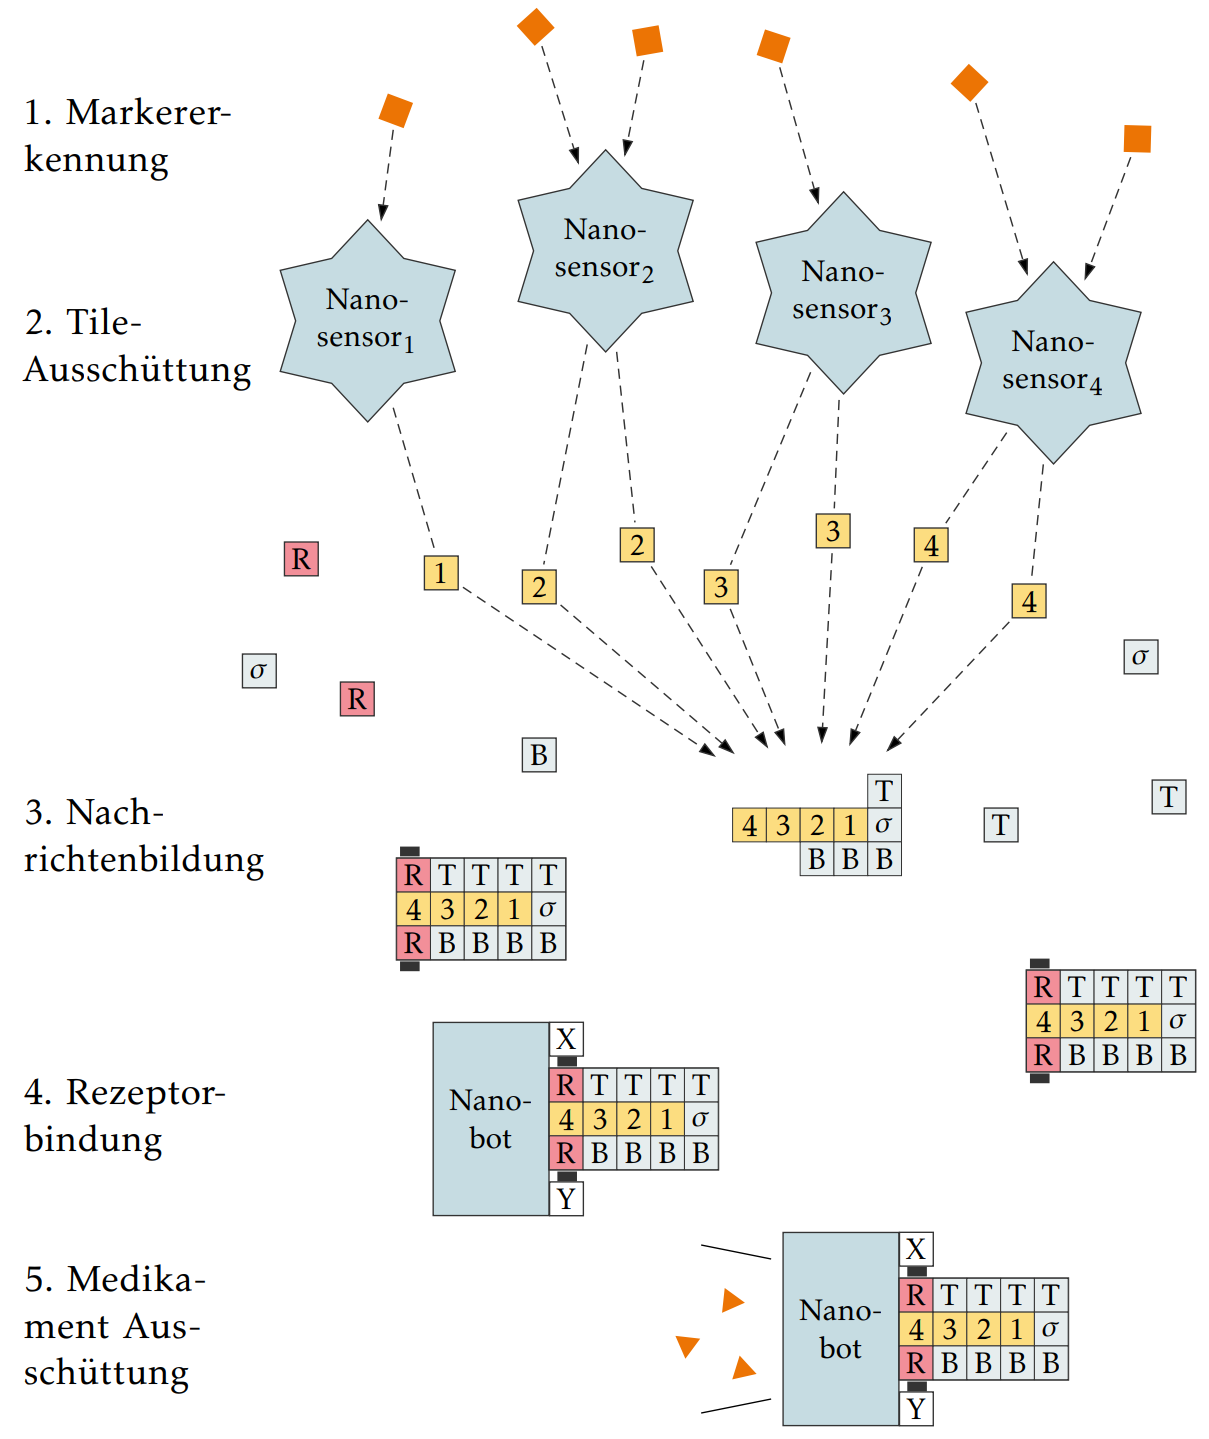
\includegraphics[width=0.9\textwidth]{images/Nanonetzwerk.png}
	\caption[Nanonetzwerk Ablauf Beispiel]{Ein beispielhafter Ablauf eines Nanonetzwerks, das ein Medikament erst dann ausschüttet, wenn vier verschiedene Sensoren Marker registriert haben. 
	Im ersten Schritt müssen Marker (hier orange) von den Nanosensoren erkannt werden, damit das System aktiviert wird. 
	Darauf folgt der zweite Schritt, in dem die Tiles ausgeschüttet werden, die zur Nachrichtenbildung benötigt werden. 
	Im dritten Schritt ist die Nachrichtenbildung dargestellt, die nur dann vollständig ist, wenn Tiles von allen vier Sensoren vorhanden sind. 
	Im vierten Schritt binden sich die Liganden der Nachricht an die Rezeptoren eines Nanoroboters. 
	Im fünften Schritt schüttet der Nanoroboter Medikamente aus, da er durch die Nachricht aktiviert wurde. \cite{lau2020phd}}
	\label{fig:nanonetzwerk_ablauf}
\end{figure}

Bei dieser Definition von DNA-basierten Nanonetzwerken ist zu beachten, dass die Nanosensoren $\mathcal{N}_{Se}$ und die Nanoroboter $\mathcal{N}_R$ korrekt aus dem Tileset $T$ gebildet werden können. 
Das muss aber nicht der Fall sein. 
In einigen Fällen kann es sinnvoller sein, die Sensoren und Roboter durch zum Beispiel DNA-Origami zu konstruieren. 
Diese Technik basiert nicht auf Tiles, sondern wie oben beschrieben auf langen DNA-Einzelsträngen und DNA-Klammern. 
Zusätzlich reduziert die eigenständige Konstruktion von Nanosensoren und Nanorobotern, beispielsweise mithilfe von DNA-Origami, die Komplexität des Tilesets $T$. 
Dementsprechend wird in dieser Arbeit der Fokus auf der Nachrichtenbildung und den dafür benötigten Tilesets liegen. 
Soweit nicht konkret von der Konstruktion von Nanosensoren oder Nanorobotern die Rede ist, wird im Folgenden bei jedem Tileset $T$ für ein Nanonetzwerk $\mathcal{N}_\Phi$ immer davon ausgegangen, dass sowohl die Nanosensoren $\mathcal{N}_{Se}$ als auch die Nanoroboter $\mathcal{N}_R$ konstruiert wurden und somit nicht im Tileset $T$ betrachtet werden müssen.

Zur Terminologie muss gesagt werden, dass hier allgemein von \emph{DNA-basierten Nanonetzwerken} gesprochen wird. Die Arbeit fokussiert sich jedoch auf die \emph{DNA-Tile-basierten Nanonetzwerke}. Das bedeutet, dass beispielsweise keine konkreten Umsetzungen von DNA-Origami-basierten Mechanismen und Geräten geliefert werden. Manchmal ist es notwendig anzunehmen, dass ein solches Gerät existiert, jedoch soll der Fokus auf den DNA-Tiles liegen.

Des Weiteren werden noch zwei neue Bausteine für die Konstruktion und Auswertung eines Nachrichtenmoleküls in einem Nanonetzwerk benötigt: \emph{Rezeptoren} und \emph{Liganden}.
Rezeptoren sind Teile eines Nanoroboters, die in der Lage sind, eine Verbindung mit Liganden einzugehen.
Liganden sind spezielle Tiles, die sich nicht nur mit einem Nachrichtenmolekül, sondern auch mit Rezeptoren eines Nanoroboters verbinden können.

Ist das Nanonetzwerk konstruiert, läuft die Kommunikation in einem solchen Netzwerk allgemein wie folgt ab:
\begin{enumerate}
	\item \emph{Markererkennung}: Die Nanosensoren des Systems können durch spezifische Marker aktiviert werden. 
	Die Art der Marker hängt von der Konstruktionsweise der Nanosensoren ab.
	Beispielsweise kann ein Nanosensor auch aus DNA-Origami gebildet werden. Durch eine Würfelform können im Inneren des Würfeln Tiles gespeichert werden. Bindet sich der Marker in Form eines DNA-Strangs, kann sich der Würfel auf einer Würfelseite öffnen.\cite{douglas2012logic}
	\item \emph{Tile-Ausschüttung}: Hat ein Nanosensor einen Marker erkannt, so schüttet dieser die Tiles aus, die zur Kommunikation im Netzwerk verwendet werden. 
	\item \emph{Nachrichtenbildung}: Die von den Sensoren freigesetzten Tiles verbinden sich durch Self-Assembly mit der bereits vorhandenen Seed-Assembly und den Liganden, um ein stabiles Nachrichtenmolekül zu bilden.
	\item \emph{Rezeptorbildung}:  Wenn die Nachricht komplett konstruiert wurde und die Liganden sich am Rand des Nachrichtenmoleküls verbunden haben, kann sich das Nachrichtenmolekül mit diesen Liganden an den Rezeptoren eines Nanoroboters binden.
	\item \emph{Nanoroboteraktivierung}: Wenn sich die Nachricht an den Rezeptoren des Nanoroboters gebunden haben, wird dieser aktiviert und erledigt die Aufgabe, für die der Nanoroboter konstruiert wurde.
\end{enumerate}

Ein Beispiel für solch eine Kommunikation ist in Abbildung~\ref{fig:nanonetzwerk_ablauf} gegeben. Hier soll ein Medikament ausgeschüttet werden, wenn vier verschiedene Sensoren ihre Marker erkennen. Dafür wird eine \glqq AND\grqq-Nachricht gebildet. 
Das Nachrichtenmolekül bildet sich nur komplett und bindet die Liganden, wenn die Tiles von allen vier Sensoren vorhanden sind. 
Diese von den Nanosensoren ausgeschütteten Tiles sind in diesem Beispiel mit \glqq 1\grqq, \glqq 2\grqq, \glqq 3\grqq\, und \glqq 4\grqq\, beschrieben.
Die Liganden sind rot mit dem Buchstaben \glqq R\grqq\, dargestellt, die Seed-Assembly durch das dafür typische $\sigma$.
Ist das Nachrichtenmolekül vollständig konstruiert, so kann es sich an den Rezeptoren (hier mit $X$ und $Y$ dargestellt) eines Nanoroboter binden.
Ist diese Verbindung fertig, wird der Nanoroboter aktiviert und lässt Medikamente aus, die dieser im Inneren gespeichert hatte.\cite{lau2020phd}

\section{Kommunikation in Nanonetzwerken}

Mit allen bis hier definierten Informationen können Nanonetzwerke erneut in Betrachtung gezogen werden. Diese Sektion wird sich auf die Kommunikation in Nanonetzwerken konzentrieren.

Die meisten Kommunikationsmethoden auf Nanoebene basieren auf \emph{Diffusion}. Dies bezeichnet die zufällige und passive Verteilung von Partikeln in einem Medium. Zu den typischen Kommunikationsmethoden, die auf diesem Prinzip aufbauen, gehören das Messen der Partikelanzahl und die Bestimmung von Konzentrationen bestimmter Partikel.
Dabei wird ein spezifischer Schwellenwert für die Partikelanzahl oder die Konzentration festgelegt, ab dem ein Ereignis als erreicht gilt. 
Wenn der Messwert den Schwellenwert überschreitet, kann dies darauf hinweisen, dass das Ereignis eingetreten ist. Es gibt jedoch Verfahren, die mehr Informationen übertragen können, aber dafür komplexere Partikelstrukturen und Messverfahren erfordern, wie das Messen von Partikeltypen und Partikelanordnungen. In solchen Fällen wird jeder Partikeltyp oder Partikelanordnung einer spezifischen Information zugeordnet. Sobald ein solcher Partikeltyp oder eine solche Anordnung durch Messungen erkannt wird, kann die entsprechende Information extrahiert werden.

In dieser Arbeit sind Tiles jedoch weiterhin die relevanteste Kommunikationsmethode. Tiles übertragen weniger Information in einem Molekül im Vergleich zum Erfassen von Partikeltypen oder -anordnungen. Allerdings ist die Bioinvasivität von Tiles deutlich geringer als bei Verfahren, die regelmäßige Messungen erfordern.\cite{farsad2016survey}

\begin{table}
	\centering
	\begin{tabular}{lll}
		\hline Problem & Signatur & Beschreibung \\\hline
		ADD & $\mathbb{Z} \times \mathbb{Z} \rightarrow \mathbb{Z}$ & Integer-Addition \\
		EQ &  $\mathbb{Z} \times \mathbb{Z} \rightarrow \{0,1\}$ & Integer-Vergleich \\
		GEQ &  $\mathbb{Z} \times \mathbb{Z} \rightarrow \{0,1\}$ & Integer-Vergleich $\geq$ \\
		LEQ &  $\mathbb{Z} \times \mathbb{Z} \rightarrow \{0,1\}$ & Integer-Vergleich $\leq$ \\
		SUB & $\mathbb{Z} \times \mathbb{Z} \rightarrow \mathbb{Z}$ & Integer-Subtraktion \\
		MULT & $\mathbb{Z} \times \mathbb{Z} \rightarrow \mathbb{Z}$ & Integer-Multiplikation \\
		DIV & $\mathbb{Z} \times \mathbb{Z} \rightarrow \mathbb{Z}$ & Integer-Division \\\hline
	\end{tabular}
	\caption[formale Problemdefinitionen]{Beispielhafte formale Definition für einige Probleme, die in Nanonetzwerken von Interesse sind. Dabei wird davon ausgegangen, dass die ganzen Zahlen binär als $\{0,1\}^k, k\in\mathbb{N}^+$ dargestellt werden.\cite{lau2020phd}}
	\label{tab:problem_definitionen}
\end{table}

Um Kommunikation mit Tiles ermöglichen zu können, müssen einige mathematische und logische Probleme algorithmisch mit Tiles gelöst werden können.
Beispiele für einige mathematische Probleme sind in Tabelle~\ref{tab:problem_definitionen} zu sehen. Diese Probleme können alle durch Self-Assembly von Tiles gelöst werden. 
Abbildung~\ref{fig:eq_bsp} zeigt beispielhaft ein Tileset sowie die resultierende Assembly für das Problem \emph{EQ}, das den Äquivalenzvergleich zweier 4-Bit Integer darstellt.
Dabei muss für die korrekte Konstruktion eine Temperatur von $\tau = 3$ angenommen werden. 

\begin{figure}
	\centering
	\begin{tikzpicture}[scale=1.2]
		\node at (0,3.25) {a)};
		% Yellow Tiles Row 1
		\tileEQSigma{1}{5.5}
		\tileEQA{2.5}{5.5}
		\tileEQB{4}{5.5}
		\tileEQC{5.5}{5.5}
		\tileEQD{7}{5.5}
		% White Tiles Row 2
		\tileEQeqNull{1}{4}
		\tileEQeqEins{2.5}{4}
		\tileEQfEinsNull{4}{4}
		\tileEQfNullEins{5.5}{4}
		% White Tiles Row 3
		\tileEQNullEins{7}{4}
		\tileEQEinsNull{8.5}{4}
		\tileEQEinsEins{10}{4}
		\tileEQNullNull{11.5}{4}
		% White Tiles Row 4
		\tileEQNotLE{1}{2.5}
		\tileEQNotUE{2.5}{2.5}
		\tileEQLE{4}{2.5}
		\tileEQUE{5.5}{2.5}
		%White Tiles Row 5 
		\tileEQNEQ{7}{2.5}
		\tileEQEQ{8.5}{2.5}
		\tileEQEn{10}{2.5}
		\tileEQEk{11.5}{2.5}
		% Red Tiles Row 6
		\tileEQUNull{1}{1}
		\tileEQUEins{2.5}{1}
		\tileEQUZwei{4}{1}
		\tileEQUDrei{5.5}{1}
		% Green Tiles Row 7
		\tileEQLNull{7}{1}
		\tileEQLEins{8.5}{1}
		\tileEQLZwei{10}{1}
		\tileEQLDrei{11.5}{1}
	\end{tikzpicture}\\\hfill\\
	\begin{tikzpicture}[scale=1.2]
		\node at (0,2.2) {b)};
		\tileEQNotUE{1}{3.4}
		\tileEQNEQ{1}{2.2}
		\tileEQNotLE{1}{1}
		%%%
		\tileEQC{2.2}{3.4}
		\tileEQEn{2.2}{2.2}
		\tileEQD{2.2}{1}
		%%%
		\tileEQUDrei{3.4}{3.4}
		\tileEQEinsEins{3.4}{2.2}
		\tileEQLDrei{3.4}{1}
		%%%
		\tileEQUZwei{4.6}{3.4}
		\tileEQfEinsNull{4.6}{2.2}
		\tileEQLZwei{4.6}{1}
		%%%
		\tileEQUEins{5.8}{3.4}
		\tileEQeqNull{5.8}{2.2}
		\tileEQLEins{5.8}{1}
		%%%
		\tileEQUNull{7}{3.4}
		\tileEQeqNull{7}{2.2}
		\tileEQLNull{7}{1}
		%%%
		\tileEQA{8.2}{3.4}
		\tileEQSigma{8.2}{2.2}
		\tileEQB{8.2}{1}
	\end{tikzpicture}
	\caption[Binärer Equivalenzvergleich auf Tile Ebene Beispiel]{Darstellung von a) dem Tileset und b) der resultierende Self-Assembly für das Problem \emph{EQ}, dem Äquivalenzvergleich zweier Integer aus Tabelle~\ref{tab:problem_definitionen}. In diesem Beispiel für 4-Bit Zahlen, lässt sich diese Konstruktion jedoch analog für beliebig lange Binärzahlen wiederholen. Das Farbschema bietet eine bessere Übersicht, wird jedoch erst im Kapitel~\ref{cha:konstruktion} notwendig. Die Binärzahlen in der Self-Assembly sind in den südlichen Kleberbezeichnern der Tiles \emph{U0}, \emph{U1}, \emph{U2} und \emph{U3} sowie in den nördlichen Kleberbezeichnern der Tiles \emph{L0}, \emph{L1}, \emph{L2} und \emph{L3} dargestellt. Die zentralen Tiles werden zur Berechnung des Problems benötigt. Von der Seed-Assembly $\sigma$ wird horizontal ein \glqq k\grqq\, in den Kleberbezeichnern weiter gegeben. Sobald eine Ziffernstelle nicht äquivalent ist, wird statt einem \glqq k\grqq\, ein \glqq n\grqq\, weitergegeben. Da in diesem Beispiel die Binärzahlen \texttt{1100} (rot) und \texttt{1000} (blau) auf Äquivalenz getestet werden, ist das Ergebnis \emph{neq} (not equal). }
	\label{fig:eq_bsp}
\end{figure}

Das Tileset und die Self-Assembly folgen dabei dem Farbschema, das im Kapitel~\ref{cha:konstruktion} definiert und benötigt wird \cite{braun2018uzlcolor}. Es wird jedoch in allen Abbildungen verwendet, da es eine einheitliche Darstellung für Assemblies bietet und neben dem später vorgestellten Nutzen auch so etwas mehr Übersicht bietet und es einfacher macht, die Abbildungen zu beschreiben.
Das gelbfarbige Tiles ist dabei die Seed-Assembly \emph{$\sigma$}. Die roten sowie blauen Tiles markieren die nördliche sowie südliche Grenze der Assembly. Dabei stellen das dunkelrote sowie dunkelblaue Tile die Liganden der Assembly dar. Das hellrote sowie hellblaue Tile stellt wiederum den \glqq Start\grqq\, der Grenze nördlich beziehungsweise südlich der Seed-Assembly dar.

In der Abbildung~\ref{fig:eq_bsp} werden die zwei zu vergleichenden Binärzahlen in den inneren Kleberbezeichnern der Tiles \emph{U0}, \emph{U1}, \emph{U2} und \emph{U3} für die erste Zahl und \emph{L0}, \emph{L1}, \emph{L2} und \emph{L3} für die zweite Zahl dargestellt.
In diesem Beispiel werden die Binärzahlen \texttt{1100} und \texttt{1000} auf Äquivalenz geprüft. 
Durch die Assembly der Tiles wird die Äquivalenz vom \emph{Least Significant Bit} (LSB) zum \emph{Most Significant Bit} (MSB) geprüft.
An den Ziffernstellen von \emph{U0} und \emph{L0} sowie von \emph{U1} und \emph{L1} ist die Berechnung noch äquivalent und es bindet sich an beiden Stellen das Tile \emph{eq0}.
Da der südliche Kleber von \emph{U2} das Label \glqq 1\grqq\,und der nördliche Kleber von \emph{L2} das Label \glqq 0\grqq\,hat, kommt es hier zur Verbindung des Tiles \emph{f10}.
Der weitere Aufbau des Moleküls folgt so nicht mehr durch weitere \emph{eq0}- oder \emph{eq1}-Tiles, da sich der horizontale Kleber in der Berechnung von \glqq k\grqq\, auf \glqq n\grqq\, ändert.
Somit bindet sich das Tile \emph{neq}. Dieses bindet nur die Liganden, die ein \glqq neq\grqq\, in den Kleberbezeichnern weitergeben.
Eine Konstruktion, wie sie in diesem Beispiel gegeben ist, funktioniert nur in aTAM fehlerfrei. 
Für kTAM, 2HAM und kTHAM könnte es sich anbieten, Snaked-Proofreading auf der Assembly zu verwenden, um Growth- oder Faceterrors zu minimieren.

Genau wie für das hier vorgestellte Äquivalenzproblem können mit dem richtigen Tileset bei einer festgelegten Temperatur $\tau$ einige mathematische und logische Probleme gelöst werden.
In Tabelle~\ref{tab:problem_definitionen} sind nur einige interessante Probleme definiert.
Eine ausführlichere Aufzählung von Problemen, die in Nanonetzwerken von Interesse sein können, findet sich in der Arbeit von Lau \cite{lau2020phd}.

Einige Routing-Protokolle lassen sich mittels Tilesets und den damit implementierten mathematischen und logischen Problemen abstrahieren. Das so vorhandene Potenzial wurde in unterschiedlichen wissenschaftlichen Arbeiten vorgestellt. Beispielsweise bedarf die in \cite{buether2018hop} beschriebene Implementierung des Hop-Count-Routings der Grundoperationen \emph{ADD, GEQ, LEQ} und \emph{EQ}. Dies veranschaulicht die Anwendbarkeit dieser Methodik und die Möglichkeiten der Problemreduktion. Einen weiteren Ansatz zeigt \cite{tsioliaridou2015corona}, in dem das Hop-Count-Routing mit noch weniger Grundoperationen umgesetzt wird. In \cite{liaskos2016routing} hingegen wird ein komplexeres Routing-Protokoll vorgestellt, das eine größere Anzahl an Operationen benötigt. Alle drei Protokolle sind im Related Work Kapitel~\ref{cha:relatedwork} genauer vorgestellt.

Diese Arbeit fokussiert sich jedoch nicht auf die konkreten mathematischen oder logischen Operationen. Eher werden Mechanismen aus herkömmlichen Kommunikationsprotokollen betrachtet und auf Nanoebene übersetzt. Dafür wichtig ist die \emph{Internationale Organisation für Normung} (ISO). Diese hat ein universelles Rahmenwerk für Kommunikationsprotokolle etabliert, das als das \emph{Open Systems Interconnection} (OSI)-Modell bekannt ist. Dieses Modell besteht aus sieben Schichten, die in zwei übergeordnete Kategorien unterteilt sind: die \emph{anwendungsorientierten Schichten} (Schichten 5-7) und die \emph{transportorientierten Schichten} (Schichten 1-4). \cite{iso1984}

Bei einer Kommunikation zwischen einem Sender und einem Empfänger, die ein dem ISO/OSI-Modell folgendes Kommunikationsprotokoll verwenden, werden diese sieben Schichten sowohl auf der Sender- als auch auf der Empfängerseite durchlaufen. Die sieben Schichten des ISO/OSI-Modells sind wie folgt:
\begin{enumerate}
	\item Bitübertragungsschicht
	\item Sicherungsschicht
	\item Vermittlungsschicht
	\item Transportschicht
	\item Kommunikationsschicht
	\item Darstellungsschicht
	\item Anwendungsschicht
\end{enumerate}

Jede Schicht des ISO/OSI-Modells bietet spezifische Dienste an und zusammen ermöglichen sie die Kommunikation und den Datenaustausch zwischen unterschiedlichen Systemen. Die Struktur und der Datenfluss durch diese Schichten sind in Abbildung~\ref{fig:osi_modell} dargestellt. Das ISO/OSI-Modell ist ein weit verbreiteter Standard für Netzwerkprotokolle. Während nicht alle Kommunikationsprotokolle strikt dem ISO/OSI-Modell folgen, verwenden zahlreiche Protokolle einige der im Modell definierten Prinzipien. Dementsprechend werden in den folgenden Untersektionen die Schichten und ihre Funktion für Nanonetzwerke vorgestellt. Dabei lassen sich alle folgenden Informationen zum ISO/OSI-Modell aus dem Buch von Tanenbaum entnehmen. \cite{tanenbaum2011computer}

\begin{figure}
	\centering
	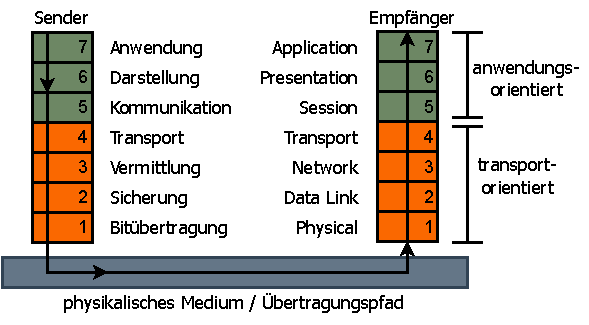
\includegraphics[width=0.7\textwidth]{images/OSI.pdf}
	\caption[OSI-Modell]{Darstellung des ISO/OSI-Modells, das eine standardisierte Kommunikation zwischen einem Sender und einem Empfänger definiert. 
	Beim Sender werden die Schichten des Modells von Anwendung, Darstellung und Kommunikation erst anwendungsorientiert durchlaufen. 
	Danach folgen die Schichten von Transport, Vermittlung, Sicherung und Bitübertragung im transportorientierten Teil. 
	Die Nachricht wird dann über das Medium an den Empfänger geschickt und in genau umgedrehter Reihenfolge entgegengenommen. Angelehnt an \cite{osi-model}.}
	\label{fig:osi_modell}
\end{figure}

\subsection{Die anwendungsorientierten Schichten}

In dieser Untersektion sollen die anwendungsorientierten Schichten des ISO/OSI-Modells näher betrachtet werden. 

Dabei ist die Anwendungsschicht im ISO/OSI-Modell die Schicht, die am nächsten an der Endbenutzer-Interaktion liegt. 
Sie ermöglicht es Anwendungen, auf das Netzwerk zuzugreifen und Dienste zu nutzen. 
Diese Schicht stellt Funktionen wie Identitätsüberprüfung, Zugangskontrolle und Ressourcenallokation zur Verfügung.

Die Darstellungsschicht im ISO/OSI-Modell kümmert sich im Wesentlichen um die Umwandlung der Daten in eine Form, die von der Anwendungsschicht verstanden werden kann. Es geht darum, wie Daten dargestellt, verschlüsselt und komprimiert werden.

Die Kommunikationsschicht spielt im ISO/OSI-Modell eine entscheidende Rolle, da sie den Datentransfer zwischen verschiedenen Netzwerken koordiniert. Sie ist zuständig für verschiedene Funktionen, wie das Routing und die Netzwerkadressierung.

Die genaue Implementierung der Mechanismen aus den anwendungsorientierten Schichten wird im Kapitel~\ref{cha:konzept} vorgestellt. Hier gibt es jedoch einige grundlegende Mechanismen, die betrachtet werden können.

Da die Anwendungsschicht durch die Benutzernähe meist eine hohe Komplexität aufweist, kann es sinnvoll sein, die Mechanismen dieser Schicht auf Mikro- statt auf Nanoebene durchzuführen. 
Am Beispiel eines In-Body-Netzwerkes kann die Aufgabe der Datenverarbeitung und der Ressourcenallokation in einem Body-Area-Netzwerk auf Mikroebene stattfinden, während das In-Body-Netzwerk sich um die niedrigeren Schichten des Modells kümmert. Dass sich unterschiedliche Netzwerktypen und Geräte um unterschiedliche Schichten des ISO/OSI-Modells kümmern, ist auch in herkömmlichen Netzwerken üblich.\cite{osi-model}

Einige Mechanismen der Darstellungsschicht sind analog in der Implementierung von Tile-basierter Self-Assembly 
enthalten. 
Ein DNA-Strang ist eine Sequenz der zwei verschiedenen Basenpaare Adenin/Thymin und Guanin/Cytosin.
So kann in einem offenen DNA-Strang, ähnlich zu einer binären Zahl, Information gespeichert und gelesen werden. Die Information, die am Ende in der Anwendungsschicht ausgelesen und genutzt werden soll, kann so in der Darstellungsschicht in die offenen DNA-Enden \glqq programmiert\grqq\, beziehungsweise codiert werden.

Auch einige Mechanismen der Kommunikationsschicht sind inhärent in Tile-basierten Self-Assemblies vorhanden. So können beispielsweise die offenen DNA-Enden der Liganden mit Adressen gleichgesetzt werden. Denn nur bestimmte Liganden können sich mit bestimmten Rezeptoren des Nachrichtenempfängers verbinden.

Ein möglicher physikalischer Prozess zur Fortbewegung ist die zuvor vorgestellte Diffusion, die beispielsweise in In-Body-Netzwerken durch den Blutfluss erzeugt wird. Andere Optionen könnten die Fortbewegung durch Flagellen oder durch molekulare Motoren sein \cite{lau2020phd}.
Wie die Mechanismen dieser Schichten in DNA-Tile-basierten Nanonetzwerken funktionieren, wird im Kapitel~\ref{cha:konzept} diskutiert. 

\subsection{Die transportorientierten Schichten}

Diese Untersektion beschäftigt sich mit den transportorientierten Schichten des ISO/OSI-Modells. Sie werden in herkömmlichen Kommunikationssystemen meist von unterschiedlichen Netzwerken oder Geräten implementiert. Dementsprechend kann für ein DNA-Tile-basiertes Nanonetzwerk nur schwer definiert werden, auf welcher Schicht der Mechanismus konkret umgesetzt wird.

Die Transportschicht des ISO/OSI-Modells ist für die End-to-End-Kommunikation und die Kontrolle des Datenflusses zwischen zwei Systemen verantwortlich.

Die Vermittlungsschicht, auch bekannt als die Datensicherungsschicht, ist im ISO/OSI-Modell dafür verantwortlich, die Kommunikation zwischen Geräten in einem Netzwerk zu kontrollieren und zu ermöglichen. Sie kümmert sich um Aufgaben wie Framing, physische Adressierung, Flusskontrolle und Fehlerkontrolle.

In der traditionellen Netzwerktechnologie stellt die Sicherungsschicht (Link Layer oder Data Link Layer im ISO/OSI-Modell) sicher, dass Daten sicher und fehlerfrei von einem Knoten zum anderen übertragen werden. Sie ist verantwortlich für die Erkennung und möglicherweise auch für die Korrektur von Fehlern, die auf der physischen Ebene auftreten können.

Die Bitübertragungsschicht, auch bekannt als die physikalische Schicht im ISO/OSI-Modell, ist für die Übertragung von rohen Bitströmen über das physische Medium zuständig. Sie befasst sich mit den technischen Aspekten der Übertragungsmedien wie Verbindungsaufbau, Verbindungstrennung, Modulation und Bitrate.

Wie zuvor angemerkt, verschwimmen die vier transportorientierten Schichten in DNA-Tile-basierten Nanonetzwerken etwas. Mechanismen zur Fehlerkorrektur sind mit dem $k \times k$-Proofreading und dem Snaked-Proofreading in der Sektion~\ref{sec:proofreading} vorgestellt worden. Mechanismen wie die Datenflusskontrolle, Framing, Fehlererkennung oder Modulation, werden im Kapitel~\ref{cha:konzept} näher betrachtet.

Dieses Kapitel hat umfassende Grundlagen von Nanonetzwerken, DNA, Tilebildung, Self-Assembly, Assembly-Modellen, Error-Handling und Kommunikationsmechanismen gebildet und geliefert. Im folgenden Kapitel werden drei Arbeiten näher betrachtet, da diese besondere Nähe zu dieser Arbeit besitzen.
